\graphicspath{{2euclid/asy/},{2euclid/pics/}}

\section{Euclidean Geometry}\label{chap:euclid}

\subsection{Euclid's Postulates and Book I of the Elements}\label{sec:euclid}

Euclid's \emph{Elements} (c.\,300\,\BC) formed a core part of European and Arabic curricula until the mid 20\th{} century. Several examples are shown below.
\begin{center}
	\newlength{\heighttt}
	\setlength{\heighttt}{100pt}
	\begin{minipage}[b]{0.35\linewidth}
		\centering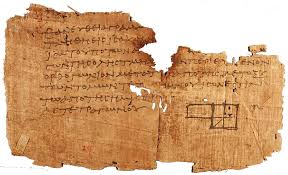
\includegraphics[height=\heighttt]{euclid1}\\
		Earliest Fragment c.\,\AD\,100
	\end{minipage}
	\begin{minipage}[b]{0.3\linewidth}
		\centering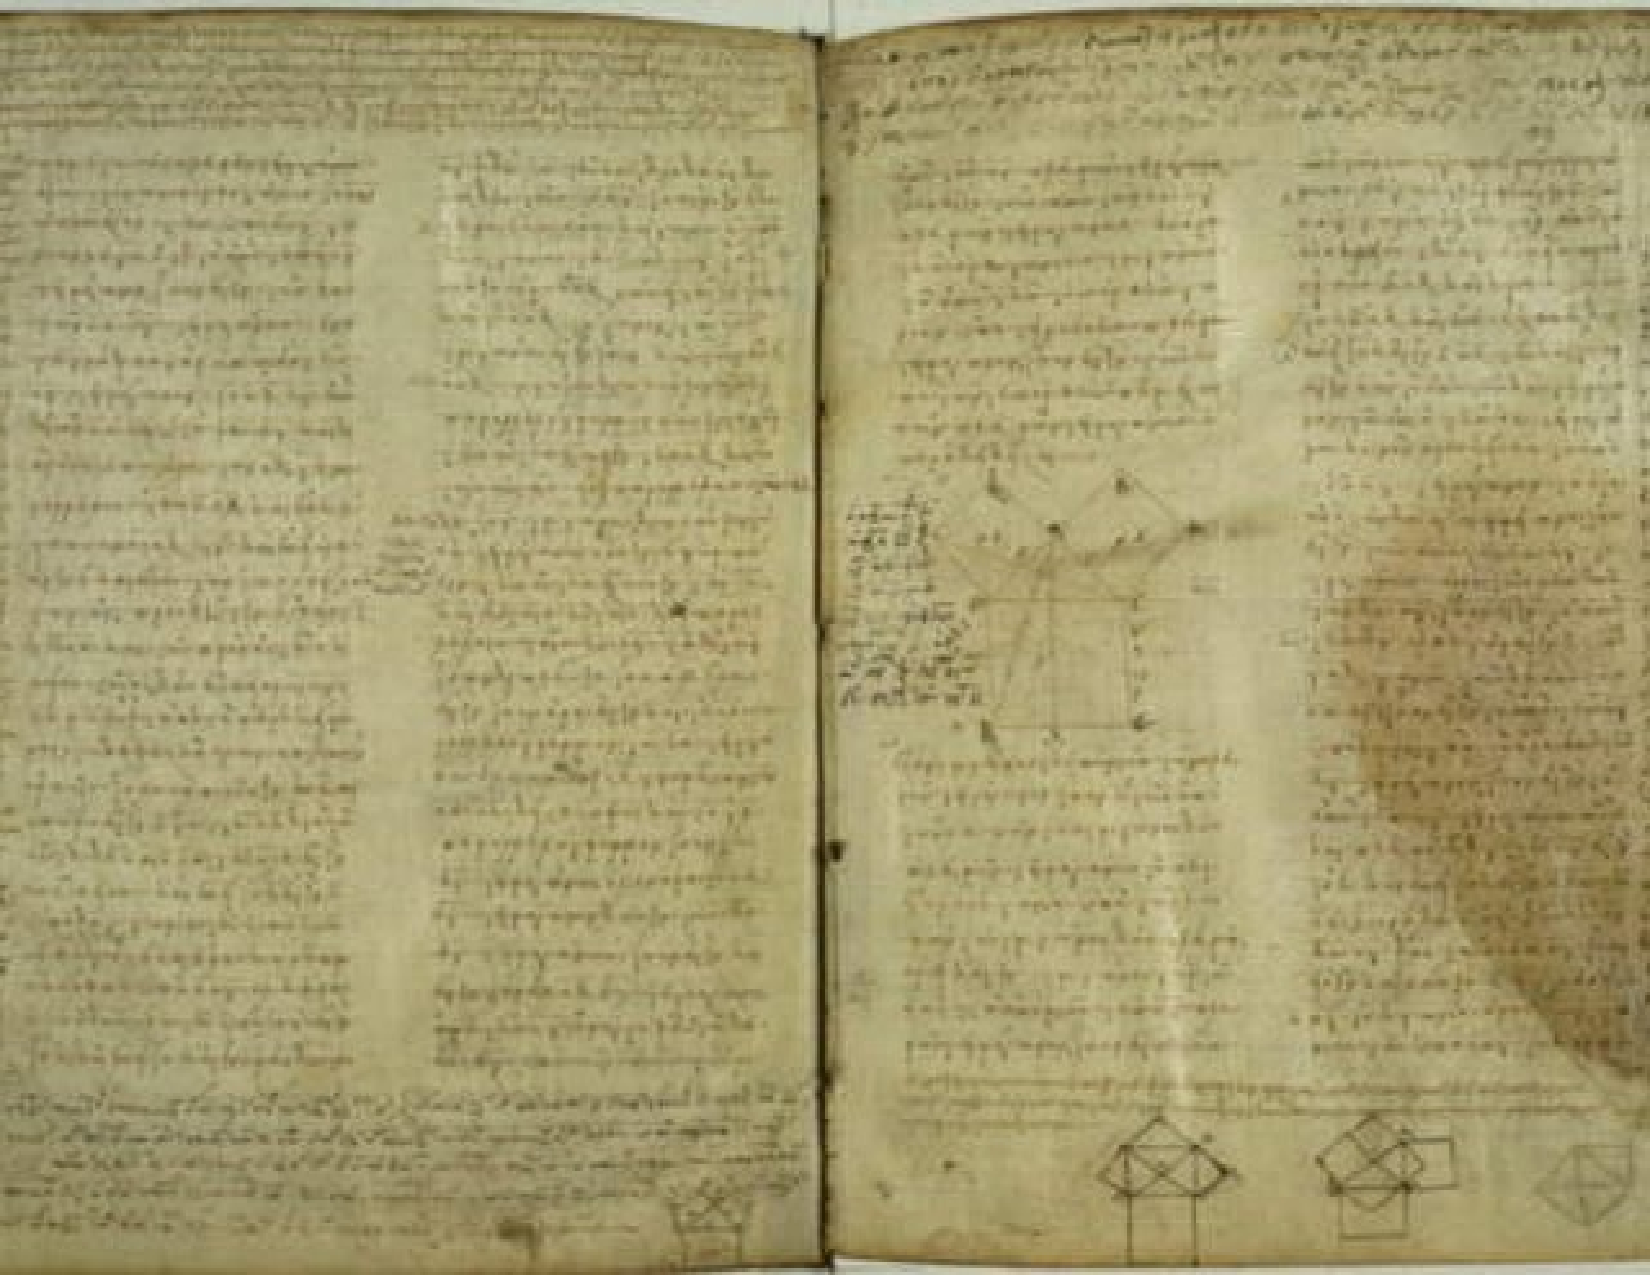
\includegraphics[height=\heighttt]{euclid2}\\
		Full copy, Vatican, 9\th\,C
	\end{minipage}
	\begin{minipage}[b]{0.33\linewidth}
		\centering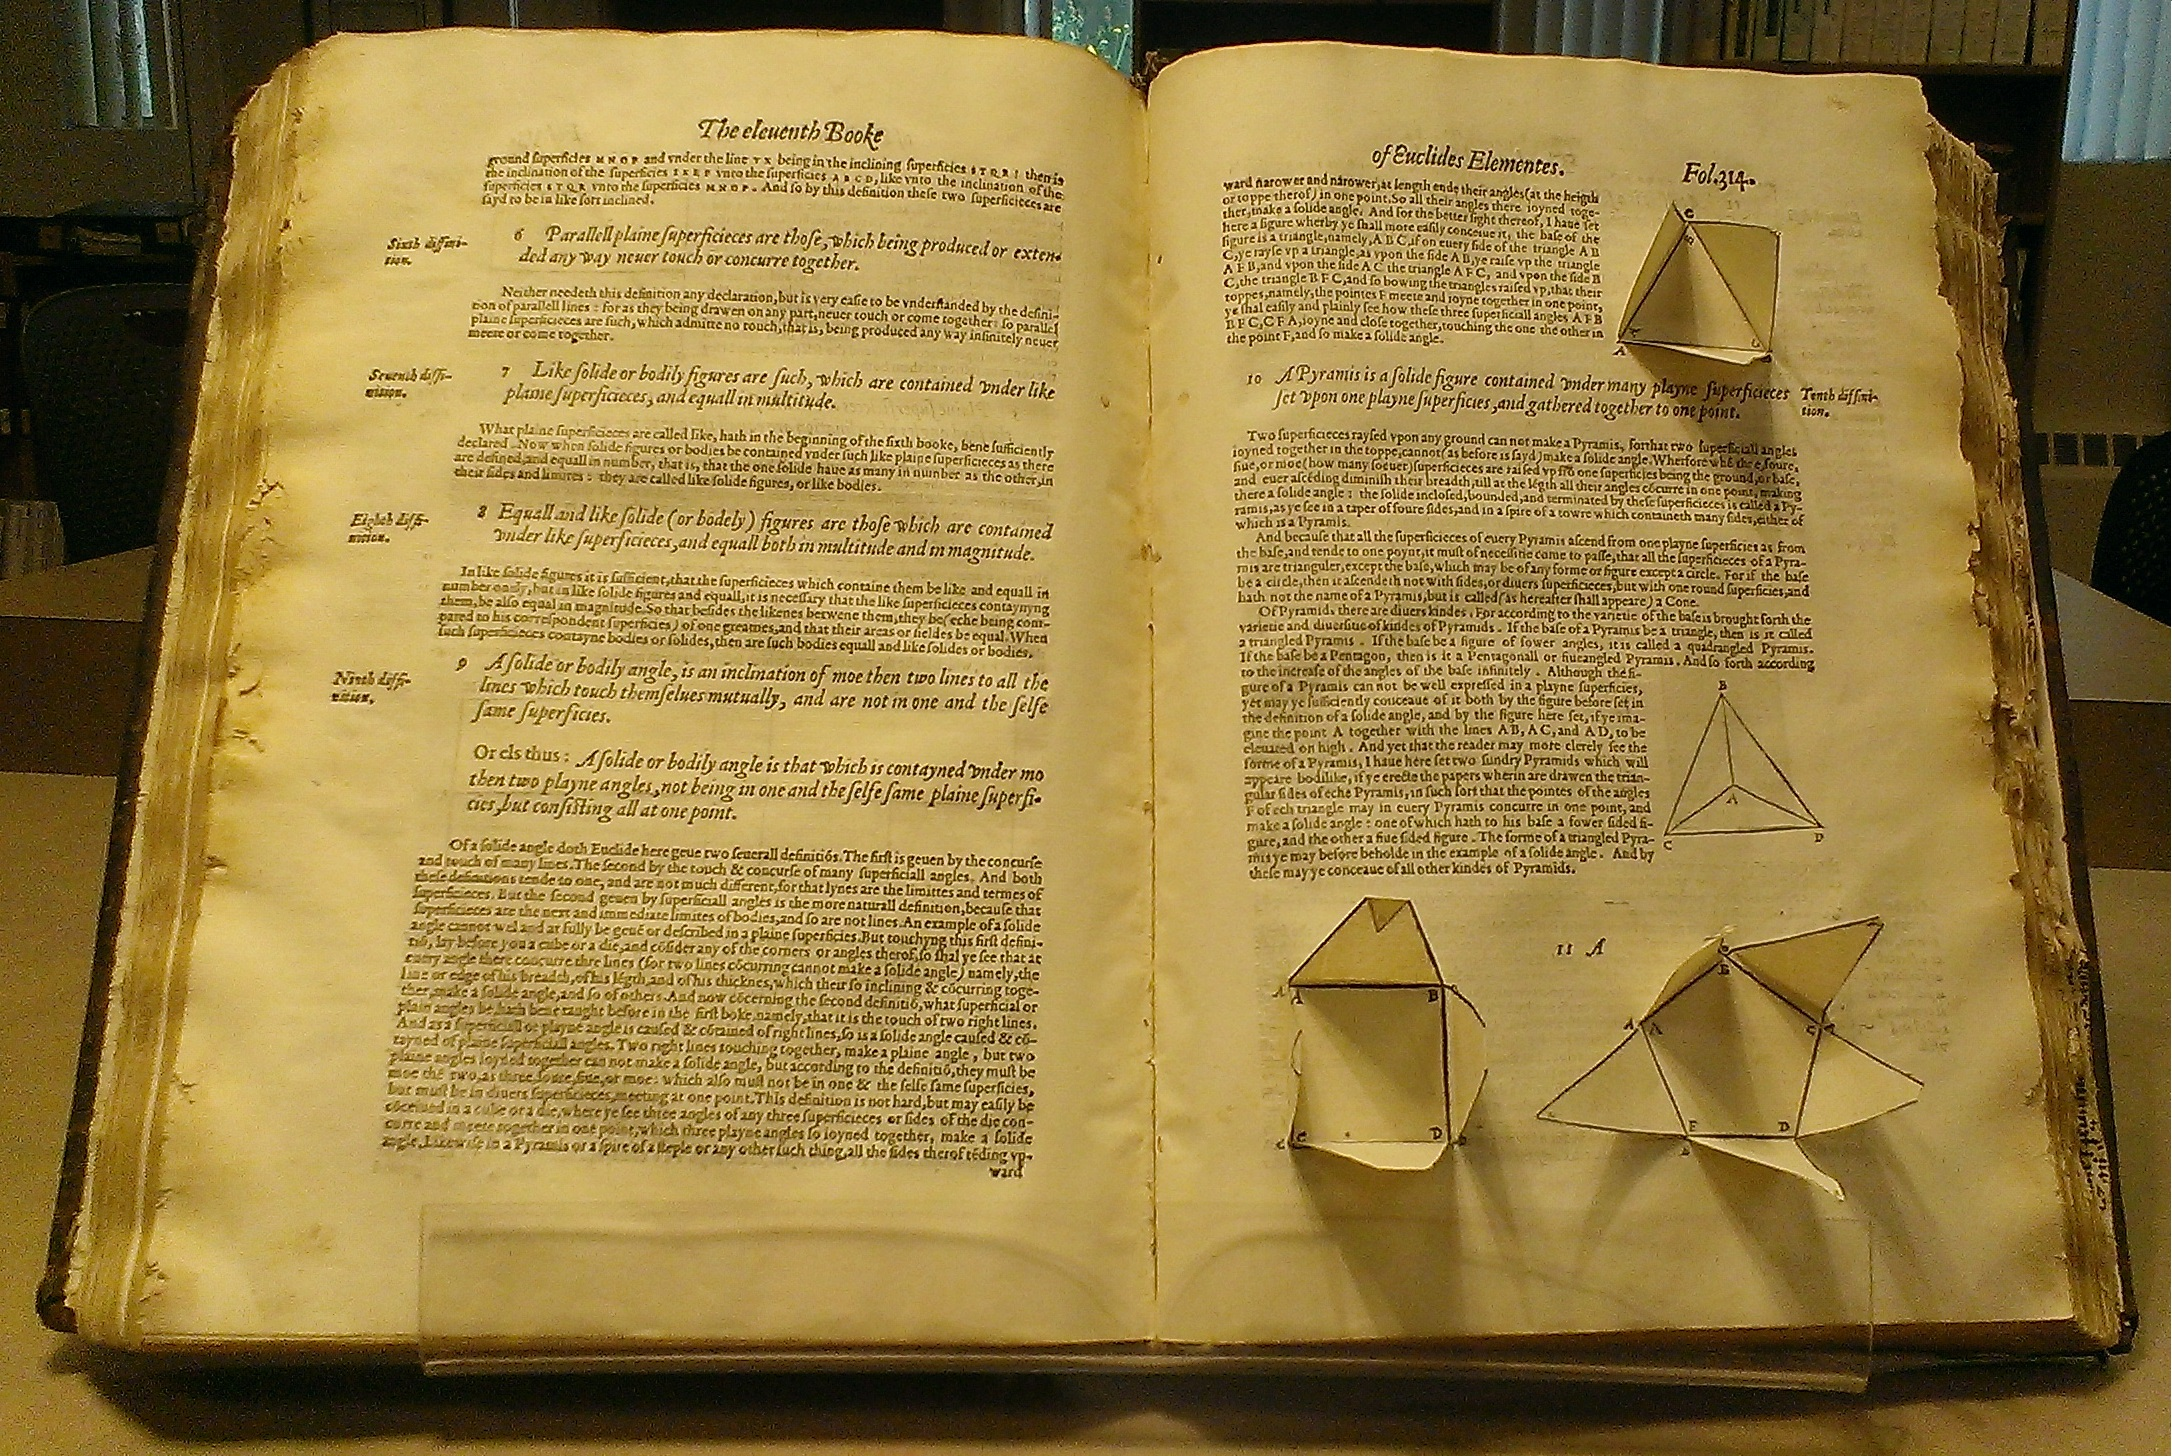
\includegraphics[height=\heighttt]{euclid3}\\
		Pop-up edition, 1500s
	\end{minipage}\\[5pt]
	\setlength{\heighttt}{135pt}
	\begin{minipage}[b]{0.44\linewidth}
		\centering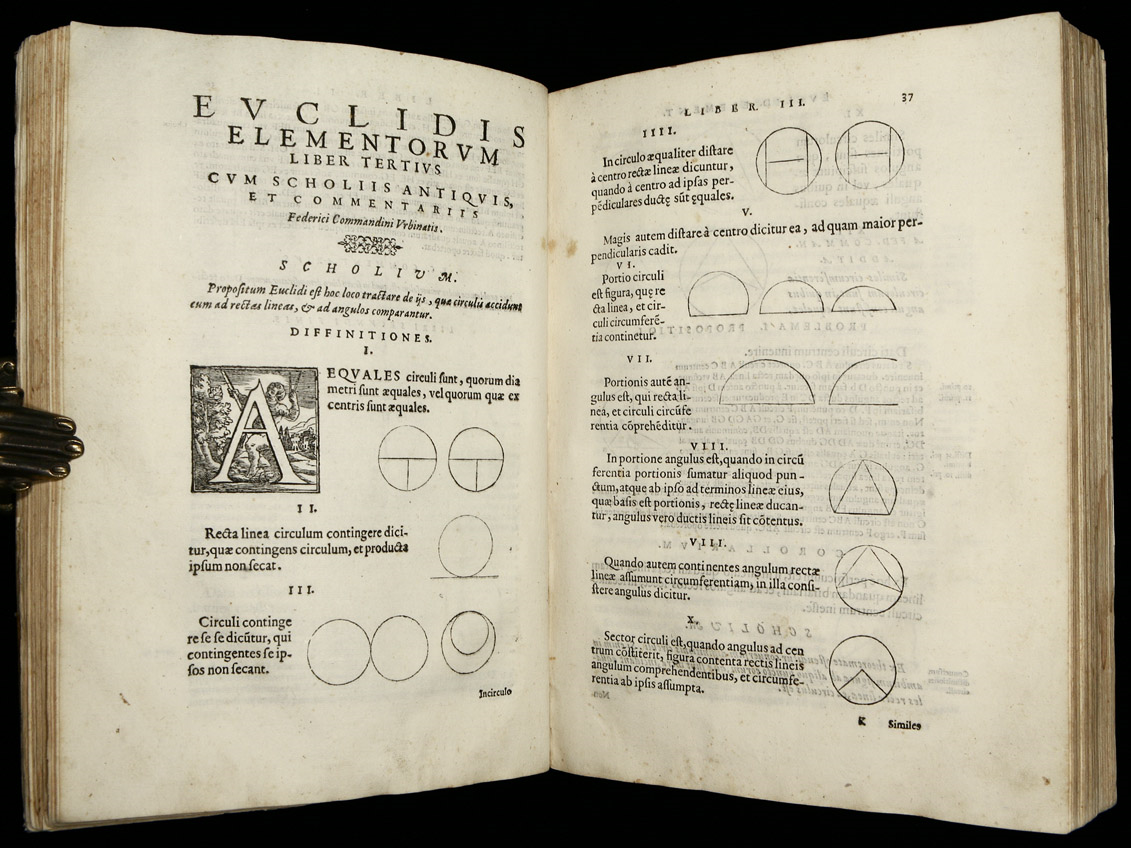
\includegraphics[height=\heighttt]{geo-09-euclid}\\
		Latin translation, 1572
	\end{minipage}
	\begin{minipage}[b]{0.3\linewidth}
		\centering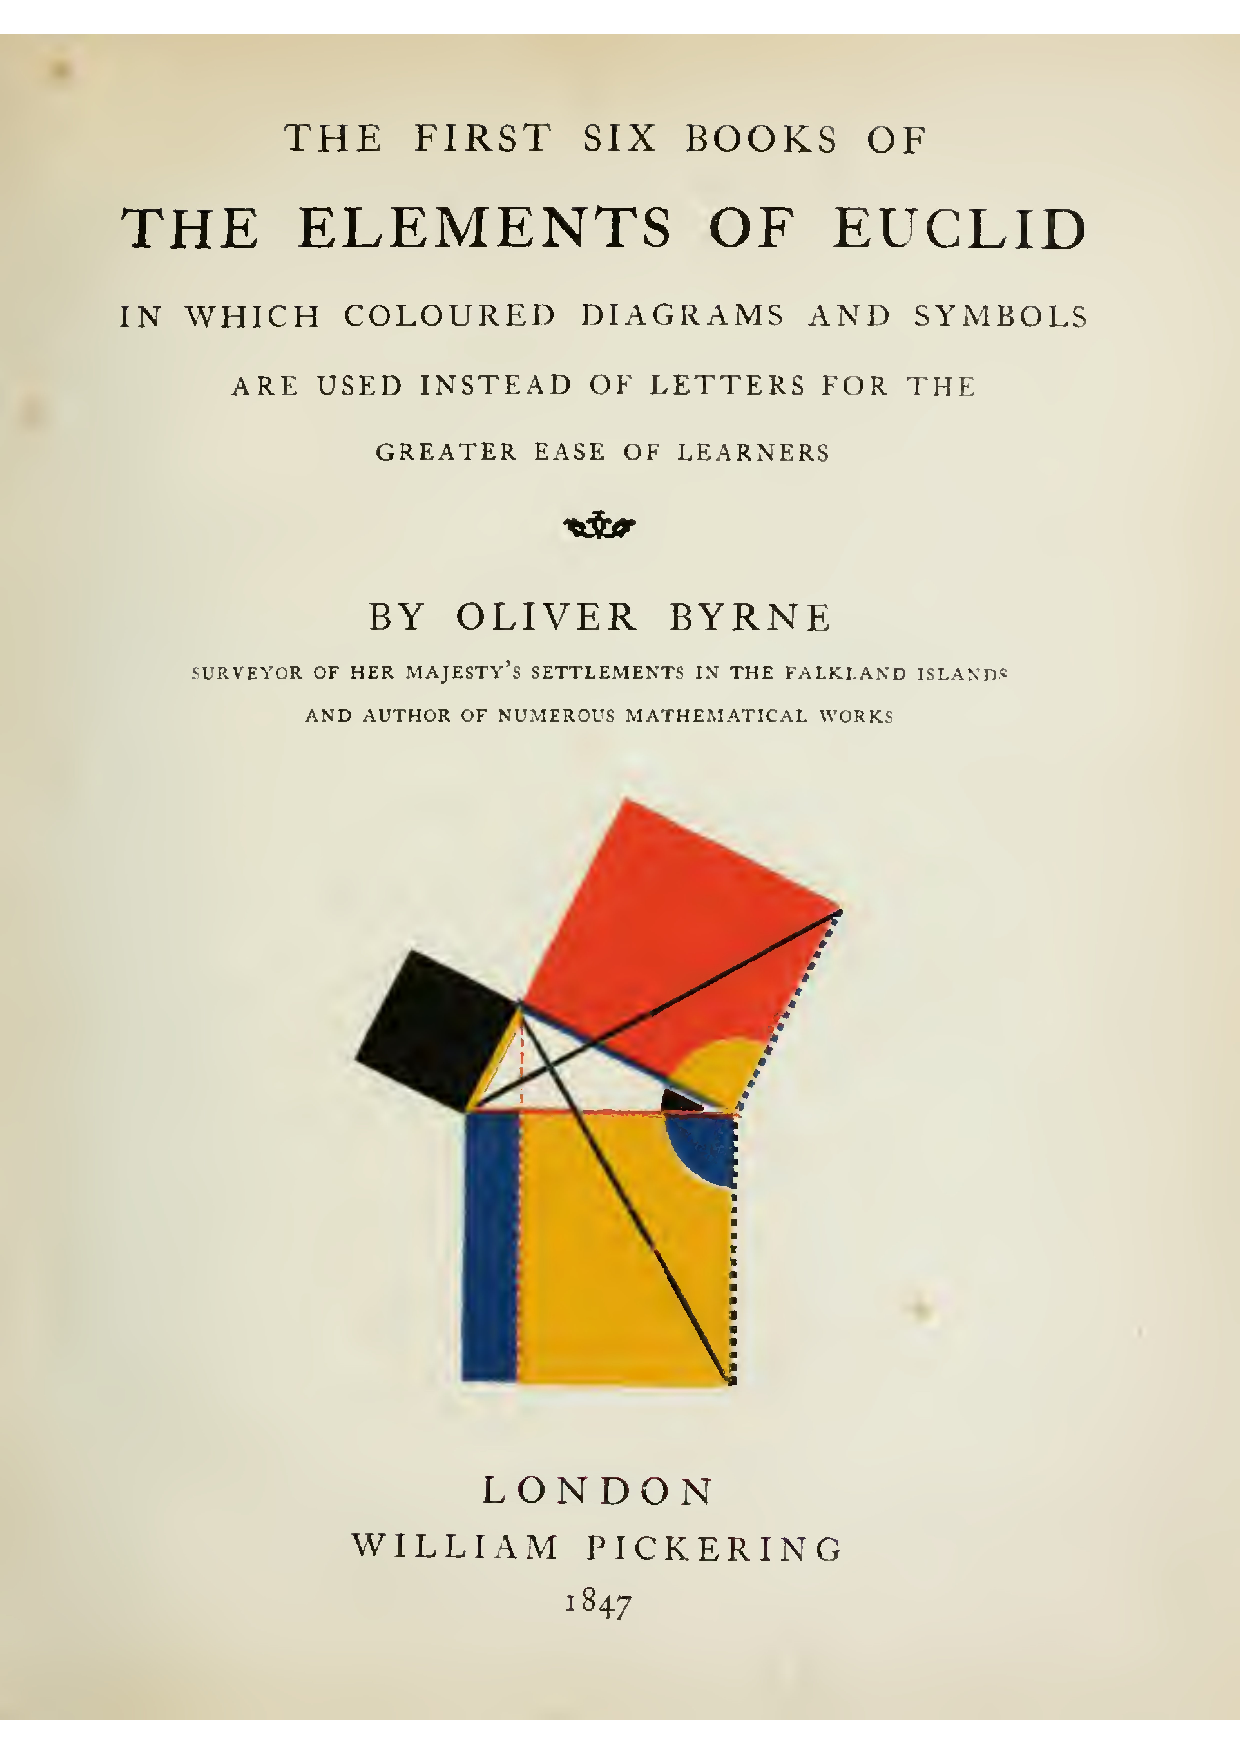
\includegraphics[height=\heighttt]{euclid5}\\
		Color edition, 1847
	\end{minipage}
	\begin{minipage}[b]{0.24\linewidth}
		\centering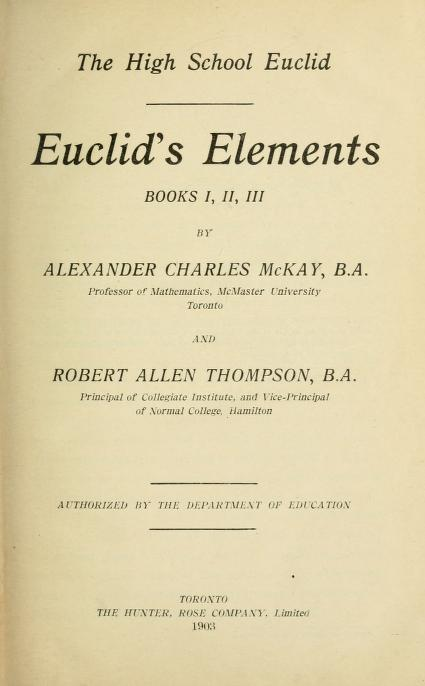
\includegraphics[height=\heighttt]{euclid4}\\
		Textbook, 1903
	\end{minipage}
\end{center}

Many of Euclid's arguments can be found \href{http://math.furman.edu/~jpoole/euclidselements/euclid.htm}{online}, and you can read Byrne's 1847 edition \href{http://math.uci.edu/~ndonalds/Elements-I-VI.pdf}{here}: the cover is Euclid's proof of Pythagoras'. We present an overview of Book I.

%to address some of the shortcomings in Euclid's original approach, it contains a more comprehensive list of definitions, has more axioms, and relabels propositions 4 and 5 as axioms (pages xviii--xxiii). 

\begin{description}\itemsep0pt
	\item[\normalfont\emph{Undefined Terms}] E.g., point, line, etc.\footnote{In fact Euclid attempted to define these: `A point is that which has no part,' and `A line has length but no breadth.'}
	\item[\normalfont\emph{Axioms/Postulates}]\negthickspace\!\footnote{In Euclid, an axiom is considered somewhat more general than a postulate. Here the postulates contain the \emph{geometry.}}\lstsp A1\lstsp If two objects equal a third, then the objects are equal\hfill ($=$ is transitive)\vspace{-5pt}
	\begin{itemize}
		\item[A2] If equals are added to equals, the results are equal\hfill ($a=c$ \& $b=d\implies a+b=c+d$)
		\item[A3] If equals are subtracted from equals, the results are equal
		\item[A4] Things that coincide are equal (in magnitude)
		\item[A5] The whole is greater than the part
		\item[P1] A pair of points may be joined to create a line
		\item[P2] A line may be extended
		\item[P3] Given a center and a radius, a circle may be drawn
		\item[P4] All right-angles are equal
		\item[P5] If a straight line crosses two others and the angles on one side sum to less than two right-angles then the two lines (when extended) meet on that side.
	\end{itemize}
\end{description}

\goodbreak

The first three postulates describe the intuitive \emph{ruler and compass constructions.} P4 allows Euclid to compare angles at different locations. P5 is usually known as the \emph{parallel postulate.}
\bigbreak

Euclid's system doesn't quite fit the modern standard. Some axioms are vague (what are `things'?) and we'll consider several more-serious shortcomings later. For now we clarify two issues and introduce some notation.
\begin{description}
	\item[\normalfont\emph{Segments}] To Euclid, a line had \emph{finite} extent; we call such a \emph{(line) segment}: the segment joining points $A,B$ is denoted $\cl{AB}$. In modern geometry, a \emph{line} extends as far as is permitted.
	\item[\normalfont\emph{Congruence}] Euclid uses \emph{equal} where modern mathematicians say \emph{congruent}. We'll express, say, congruent angles as $\angle ABC\cong\angle DEF$ rather than $\angle ABC=\angle DEF$.
\end{description}


\boldsubsubsection{Basic Theorems à la Euclid}

Theorems were typically presented as a \emph{problem}; Euclid first provides a construction (P1--P3) before proving that his construction solves the problem.

\begin{thm}{I.\,1}{}
	Problem: to construct an equilateral triangle on a given segment.
\end{thm}

The labelling I.\,1 indicates Book I, Theorem 1.

\begin{tcolorbox}[proofstyle, lower separated=false, sidebyside, sidebyside align=top seam, sidebyside gap=0pt, righthand width=0.35\linewidth]
	\emph{Proof.}\ \ Given a line segment $\cl{AB}$:\smallbreak
	By P3, construct circles centered at $A$ and $B$ with radius $\cl{AB}$.\smallbreak
	Call one of the intersection points $C$; by P1, construct $\cl{AC}$ and $\cl{BC}$.\smallbreak
	We claim that $\triangle ABC$ is equilateral.\medbreak
	Observe that $\cl{AB}$ and $\cl{AC}$ are radii of the circle centered at $A$, while $\cl{AB}$ and $\cl{BC}$ are radii of the circle centered at $B$. By Axiom A1, the three sides of $\triangle ABC$ are congruent.
	\tcblower
	\flushright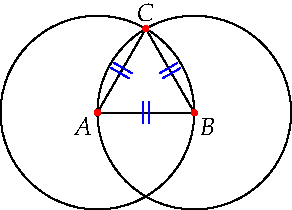
\includegraphics{euclid-I1}\hfil\qedsymbol
\end{tcolorbox}


Euclid proceeds to develop several well-known constructions and properties of triangles.
\begin{itemize}\itemsep0pt
  \item (I.\,4) Side-angle-side (SAS) congruence: if two triangles have two pairs of congruent sides and the angles between these are congruent, then the remaining sides and angles are congruent in pairs.
  \[
  	\begin{cases}
		  \cl{AB}\cong\cl{DE}\\
		  \angle ABC\cong\angle DEF\\
		  \cl{BC}\cong\cl{EF}
 	 	\end{cases}
  	\quad\implies
  	\begin{cases}
		  \cl{AC}\cong\cl{DF}\\
		  \angle BCA\cong\angle EFD\\
		  \angle CAB\cong\angle FDE
  	\end{cases}
  \]
  \item (I.\,5) An isosceles triangle has congruent base angles.
  \item (I.\,9) To bisect an angle.
  \item (I.\,10) To find the midpoint of a segment.
  \item (I.\,15) If two lines/segments cut one another, opposite angles are congruent.
\end{itemize}
Have a look at some of Euclid's arguments online. These are worth reading despite there being logical issues with Euclid's presentation. We'll revisit these results in the Exercises and next two sections. 

\goodbreak


\boldsubsubsection{Parallel Lines: Construction \& Existence}

\begin{defn}{}{parallel}
	Lines are \emph{parallel} if they do not intersect. Segments are parallel if no extensions of them intersect.
\end{defn}

In Euclid, a line is not parallel to itself. The next result is one of the most important in Euclidean geometry; it describes how to create a parallel line through a given point.


\begin{thm}[lower separated=false, sidebyside, sidebyside align=top seam, sidebyside gap=0pt, righthand width=0.37\linewidth]{I.\,16\ Exterior Angle Theorem}{extangle}
	If one side of a triangle is extended, then the exterior angle is larger than either of the opposite interior angles.\smallbreak
	In the picture, we have $\delta>\alpha$ and $\delta>\beta$.
	\tcblower
	\flushright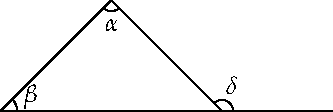
\includegraphics{euclid-I16}
\end{thm}

Euclid did not quantify angles numerically: $\delta>\alpha$ means that $\alpha$ is congruent to some angle \emph{inside} $\delta$.

\begin{proof}
	Construct the bisector $\cl{BM}$ of $\cl{AC}$ \ (I.\,10).\par
	\begin{minipage}[t]{0.64\linewidth}\vspace{-5pt}
		Extend $\cl{BM}$ to $E$ such that $\cl{BM}\cong\cl{ME}$ \  (I.\,2) and connect $\cl{CE}$ \  (P1).\smallbreak
		The opposite angles at $M$ are congruent \ (I.\,15).\smallbreak
		SAS (I.\,4) applied to $\triangle AMB$ and $\triangle CME$ says $\angle BAM\cong\angle EMC$, which is clearly smaller than the exterior angle at $C$.
	\end{minipage}
	\hfill
	\begin{minipage}[t]{0.35\linewidth}\vspace{-20pt}
		\flushright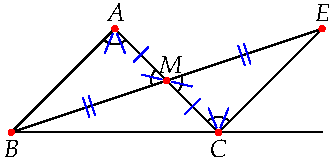
\includegraphics{euclid-I16p}
	\end{minipage}
	\smallbreak
	Bisect $\cl{BC}$ and repeat the argument to see that $\beta<\delta$.
\end{proof}

The proof in fact \emph{constructs} a parallel ($\cl{CE}$) to $\cl{AB}$ through $C$, as the next result shows.

\begin{thm}[lower separated=false, sidebyside, sidebyside align=top seam, sidebyside gap=0pt, righthand width=0.32\linewidth]{I.\,27}{}
	If a line falls on two other lines such that the alternate angles ($\alpha,\beta$) are congruent, then the two lines are parallel.
	\tcblower
	\flushright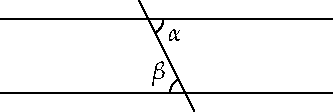
\includegraphics{euclid-I27}
\end{thm}

The \emph{alternate angles} in the exterior angle theorem are those at $A$ and $C$: $\cl{CE}$ really is parallel to $\cl{AB}$.

\begin{tcolorbox}[proofstyle,lower separated=false, sidebyside, sidebyside align=top seam, sidebyside gap=0pt, righthand width=0.37\linewidth]
	\emph{Proof.}\lstsp If the lines were not parallel, they would meet on one side. WLOG suppose they meet on the right side at $C$.\smallbreak
	The angle $\beta$ at $B$, being exterior to $\triangle ABC$, must be greater than the angle $\alpha$ at $A$ \ (I.\,16): contradiction.
	\tcblower
	\flushright
	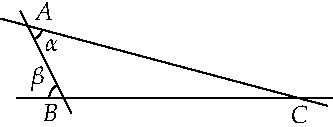
\includegraphics{euclid-I27p}\\[-12pt]\hfill\qedsymbol
\end{tcolorbox}

Euclid combines this with the vertical angles theorem (I.\,15) to finish the first half of Book I.

\begin{cor}[lower separated=false, sidebyside, sidebyside align=top seam, sidebyside gap=0pt, righthand width=0.32\linewidth]{I.\,28}{}
	If a line falling on two other lines makes congruent angles, then the two lines are parallel.
	\tcblower
	\flushright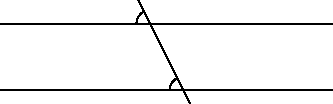
\includegraphics{euclid-I28}
\end{cor}


Thus far, Euclid uses only postulates P1--P4. In any model in which these hold:
\[
	\tcbhighmath{\text{Given a line $\ell$ and a point $C$ not on $\ell$, \textbf{there exists} a parallel to $\ell$ through $C$}}
\]
\goodbreak


\boldsubsubsection{Parallel Lines: Uniqueness, Angle-sums \& Playfair's Postulate}


Euclid finally invokes the parallel postulate to prove the converse of I.\,27, showing that the congruent alternate angle approach is the \emph{only} way to have parallel lines.

\begin{thm}{I.\,29}{}
	If a line falls on two parallel lines, then the alternate angles are congruent.
\end{thm}

\begin{tcolorbox}[proofstyle,lower separated=false, sidebyside, sidebyside align=top seam, sidebyside gap=0pt, righthand width=0.37\linewidth]
	\emph{Proof.}\ \ Given the picture, we must prove that $\alpha\cong\beta$.\smallbreak
	Suppose not and WLOG that $\alpha>\beta$.\smallbreak
	But then $\beta+\gamma<\alpha+\gamma$, which is a straight edge.\smallbreak
	By the parallel postulate, the lines $\ell,m$ meet on the left side of the picture, whence $\ell$ and $m$ are not parallel.
	\tcblower
	\flushright
	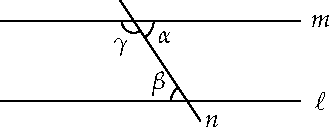
\includegraphics{euclid-I29}\\[-10pt]\qedsymbol
\end{tcolorbox}

The most well-known result about triangles is now in our grasp; the interior angles sum to a straight edge. Euclid words this slightly differently.

\begin{thm}{I.\,32}{}
	If one side of a triangle is extended, the exterior angle is congruent to the sum of the opposite interior angles.
\end{thm}

\begin{minipage}[t]{0.62\linewidth}\vspace{-4pt}
	\emph{This is not a numerical sum,} though for familiarity's sake we'll often write \ang{180} for a straight edge and \ang{90} for a right-angle.\par
	In the picture we've labelled angles as Greek letters for clarity. The result amounts to showing that $\widetilde\alpha+\widetilde\beta\cong\alpha+\beta$.
\end{minipage}
\hfill
\begin{minipage}[t]{0.37\linewidth}\vspace{-9pt}
	\flushright
	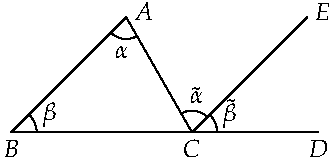
\includegraphics{euclid-I32}
\end{minipage}

\vspace{-20pt}

\begin{proof}
	Construct $\cl{CE}$ parallel to $\cl{BA}$ as in I.\,16, so that $\widetilde\alpha\cong\alpha$.\smallbreak
	$\cl{BD}$ falls on parallel lines $\cl{AB}$ and $\cl{CE}$, whence $\widetilde\beta\cong\beta$ (Corollary of I.\,29).\smallbreak
	Axiom A2 shows that $\angle ACD=\widetilde\alpha+\widetilde\beta\cong\alpha+\beta$.
\end{proof}


\medskip


The parallel postulate is stated in the negative (angles \emph{don't} sum to a straight edge, therefore lines are \emph{not} parallel). Though we cannot be sure, Euclid possibly chose this formulation in order to facilitate proofs by contradiction. Unfortunately the effect is to obscure the meaning of the parallel postulate. Here is a more modern interpretation.

\begin{axiom}[lower separated=false, sidebyside, sidebyside align=top seam, sidebyside gap=0pt, righthand width=0.37\linewidth]{Playfair's Postulate}{playfair}
	Given a line $\ell$ and a point $C$ not on $\ell$, \textbf{at most one} parallel line $m$ to $\ell$ passes through $C$.
	\tcblower
	\flushright
	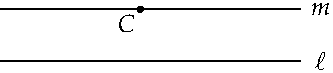
\includegraphics{euclid-playfair-defn}
\end{axiom}


\begin{minipage}[t]{0.62\linewidth}\vspace{0pt}
	Our discussion up to now shows that the parallel postulate implies Playfair.
	\begin{itemize}\itemsep0pt
	  \item Let $A,B\in\ell$ and construct the triangle $\triangle ABC$.
	  \item The exterior angle theorem constructs $E$ and thus a parallel $m$ to $\ell$ by I.\,27.
	  \item I.\,29 invokes the parallel postulate to prove that this is the \emph{only} such parallel.
	\end{itemize}
\end{minipage}
\hfill
\begin{minipage}[t]{0.37\linewidth}\vspace{0pt}
	\flushright
	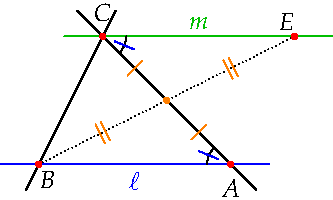
\includegraphics{euclid-playfair3}
\end{minipage}\bigbreak

In fact the postulates are equivalent.

\begin{thm}{}{}
	In the presence of Euclid's first four postulates, Playfair's postulate and the parallel postulate (P5) are equivalent.
\end{thm}

\begin{proof}
	\begin{description}
		\item[\normalfont (P5 $\Rightarrow$ Playfair)] We proved this above.
		\item[\normalfont (Playfair $\Rightarrow$ P5)] We prove the contrapositive. Assume postulates P1--P4 are true and that P5 is \emph{false.} Using quantifiers, and with reference to the picture in I.\,29, we restate the parallel postulate:
	\begin{quote}
	  P5:\lstsp $\forall$ pairs of lines $\ell,m$ and $\forall$ crossing lines $n$, \  $\beta+\gamma<\ang{180}\implies\ell,m$ \emph{not parallel.}
	\end{quote}
	\begin{minipage}[t]{0.62\linewidth}\vspace{-7pt}
		Its \emph{negation} (P5 false) is therefore:
		\begin{quote}
	  	$\exists$ parallel lines $\ell,m$ and a crossing line $n$ for which $\beta+\gamma<\ang{180}$
		\end{quote}
		This is without loss of generality: if $\beta+\gamma>\ang{180}$, consider the angles on the other side of $n$.\medbreak
		By the the exterior angle theorem/I.\,28, we may build a parallel line $\hat\ell$ to $\ell$ through the intersection $C$ of $m$ and $n$: in the picture, $\hat\beta\cong\beta$. Crucially, this only requires postulates P1--P4!
	\end{minipage}
	\hfill
	\begin{minipage}[t]{0.37\linewidth}\vspace{0pt}
		\flushright
		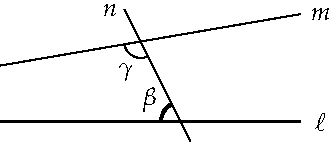
\includegraphics{euclid-playfair2}\\
		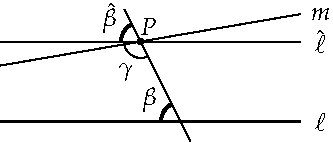
\includegraphics{euclid-playfair}
	\end{minipage}\smallbreak
	Observe that $\hat\ell$ and $m$ are \emph{distinct} since $\hat\beta+\gamma\cong\beta+\gamma<\ang{180}$.
	We therefore have a line $\ell$ and a point $C$ not on $\ell$, though which pass (at least) \emph{two} parallels to $\ell$: Playfair's postulate is \emph{false.} \qedhere
	\end{description}
\end{proof}



\boldsubsubsection{Non-Euclidean Geometry}\phantomsection\label{pg:sphere}

That Euclid waited so long before invoking the uniqueness of parallels suggests he was trying to establish as much as he could about triangles and basic geometry in its absence. By contrast, everything from I.\,29 onwards relies on the parallel postulate, including the proof that the angle sum in a triangle is \ang{180}. For centuries, many mathematicians believed, though none could prove it, that such a fundamental fact about triangles must be true independent of the parallel postulate.\smallbreak
Loosely speaking, a \emph{non-Euclidean geometry} is a model for which a parallel through an off-line point either doesn't exist or is non-unique. It wasn't until the 17--1800s and the development of \emph{hyperbolic geometry} (Chapter \ref{chap:hyper}) that a model was found in which Euclid's first four postulates hold but for which the parallel postulate is false.\footnote{This shows that the parallel postulate is independent: in fact all Euclid's postulates are independent. They are also consistent (the `usual' points and lines in the plane are a model), but incomplete: a sample undecidable is in Exercise \ref{ex:euclidundecideable}.}\par

\begin{minipage}[t]{0.76\linewidth}\vspace{-5pt}
	We shall eventually see that every triangle in hyperbolic geometry has angle sum less than \ang{180}, though this will require a lot of work! For a more easily visualized non-Euclidean geometry consider the sphere. A rubber band stretched between three points on its surface describes a \emph{spherical triangle}; an example with angle sum \ang{270} is drawn. A similar game can be played on a saddle-shaped surface: as in hyperbolic geometry, `triangles' will have angle sum less than \ang{180}.
\end{minipage}
\hfill
\begin{minipage}[t]{0.23\linewidth}\vspace{-10pt}
	\flushright
	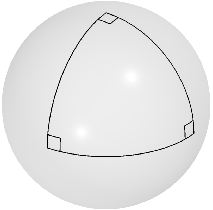
\includegraphics[scale=0.95]{euclid-sphere}
\end{minipage}

\goodbreak

\goodbreak


\boldsubsubsection{Pythagoras' Theorem}

Following his discussion of parallels, Euclid shows that parallelograms with the same base and height are equal (in area) (I.\,33--41), before providing explicit constructions of parallelograms and squares (I.\,42--46). Some of this is covered in Exercise \ref{ex:pythagexs}. Immediately afterwards comes the capstone of Book I.


\begin{thm}{I.\,47 Pythagoras' Theorem}{}
	The square on the hypotenuse of a right triangle equals (has the same area as) the sum of the squares on the other sides.
\end{thm}

\begin{proof} 
	The given triangle $\triangle ABC$ is assumed to have a right-angle at $A$.\par
	\begin{minipage}[t]{0.6\linewidth}\vspace{0pt}
	\begin{enumerate}\itemsep0pt
	  \item Construct squares on each side of $\triangle ABC$ \ (I.\,46) and a parallel $\cl{AL}$ to $\cl{BD}$ \ (I.\,16).
	  \item $\cl{AB}\cong\cl{FB}$ and $\cl{BD}\cong\cl{BC}$ since sides of squares are congruent. Moreover $\angle ABD\cong\angle FBC$ since both contain \textcolor{blue}{$\angle ABC$} and a \textcolor{red}{right-angle}.
	  \item Side-angle-side (I.\,4) says that $\triangle ABD$ and $\triangle FBC$ are congruent (identical up to rotation by \ang{90}).
		\item I.\,41 compares areas of parallelograms and triangles with the same base and height:\vspace{0pt}
		\begin{align*}
			\operatorname{Area}(\textcolor{red}{\square ABFG})&=2\operatorname{Area}(\triangle FBC)\\
			&=2\operatorname{Area}(\triangle ABD)\\
			&=\operatorname{Area}\left(\textcolor{red}{\fbox{\phantom{'}}BOLD}\right)\\[-25pt]
		\end{align*}
		\item Similarly $\operatorname{Area}(\textcolor{Green}{\square ACKH}) =\operatorname{Area}\left(\textcolor{Green}{\fbox{\phantom{'}}OCEL}\right)$.
	\end{enumerate}
	\end{minipage}
	\hfill
	\begin{minipage}[t]{0.39\linewidth}\vspace{0pt}
		\flushright
		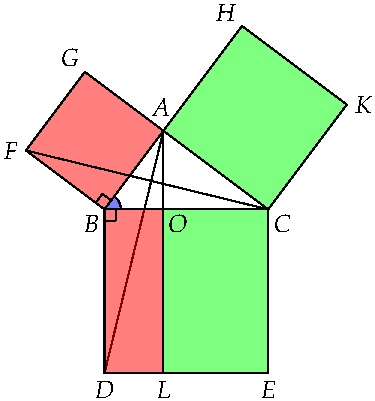
\includegraphics{euclid-I47}
	\end{minipage}
	\begin{enumerate}\setcounter{enumi}{5}
		\item Sum the rectangles to obtain $\square BCED$ and complete the proof.\hfill\qedhere
	\end{enumerate}
\end{proof}



Euclid finishes Book I with the converse, which we state without proof.

\begin{thm}{I.\,48}{}
	If the (areas of the) squares on two sides of a triangle equal the (area of the) square on the third side, then the  triangle has a right-angle opposite the third side.
\end{thm}

Euclid's argument is very sneaky, and absolutely worth looking up!\bigbreak

The \emph{Elements} contains thirteen books. Much of the remaining twelve discuss further geometric constructions, including in three dimensions. There is also a healthy dose of basic number theory including what is now known as the Euclidean algorithm. This is enough pure Euclid for us however; we now turn to a more modern description, courtesy of David Hilbert.

\clearpage

% 
% \paragraph{Book II: Geometric algebra}
% 
% We tend to think of Pythagoras' Theorem as a statement in Geometric Algebra: i.e., $c^2=a^2+b^2$, but this is not how Euclid saw it. To Euclid, Geometric Algebra was about solving equations to find unknowns. Of course the concept of algebra hadn't been invented yet, so the very problems had to be stated geometrically. Such concerns comprise the bulk of Book II of the \emph{Elements,} and are mostly attributable to the Pythagoreans.Here is an example.
% 
% \begin{thm*}[II.\,11]
% A straight line can be divided so that the rectangle contained by the whole and one of the segments is equal to the square on the remaining segment.
% \end{thm*}
% 
% 
%  In our modern language we would say: given $AB=a$, find $H$ on $AB$, so that $AH=x$, with $x^2=a(a-x)$. Here is Euclid's proof.
% 
% \begin{minipage}{0.3\textwidth}
% 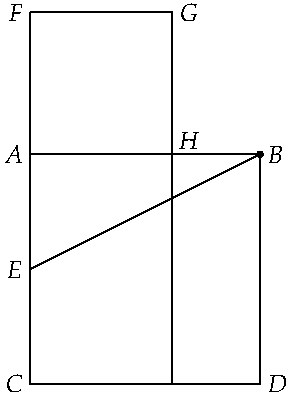
\includegraphics{geo-17-bk2}
% \end{minipage}\hfill
% \begin{minipage}{0.6\textwidth}
% \begin{enumerate}
%   \item Construct square $ABDC$ on $AB$
% 	\item Bisect $AC$; call midpoint $E$
% 	\item Connect $EB$
% 	\item Extend $AC$
% 	\item Lay off $EF=EB$ on $AC$ extended
% 	\item Construct square $FGHA$
% \end{enumerate}
% \end{minipage}
% 
%  In our modern language, with our understanding of Pythagoras', we see that Euclid has constructed $H$ so that $x=\frac{\sqrt 5-1}2a$. We can easily check that this solves the equation $x^2=a(a-x)$. Note that this is a construction of the golden ratio:
% \[AH:HB=1:\frac{\sqrt 5-1}2=\frac{\sqrt 5+1}2:1.\]
% For many centuries after Euclid, the meaning of `solve' was exactly this: construct a solution.


\begin{exercises}
	\hangindent\doubleind
	1. \ (a) \ Prove the \emph{vertical angle theorem} (I.\,15): if two lines cut one another, opposite angles are congruent.\vspace{-8pt}

	\begin{enumerate}\setcounter{enumi}{1}
	  \item[]\begin{enumerate}\setcounter{enumii}{1}
	    \item[](\emph{Hint: This is one place where you will need to use postulate 4 regarding right-angles})
	    \item Use part (a) to complete the proof of the exterior angle theorem: i.e.\ explain why $\beta<\delta$.
	  \end{enumerate}
	
		\item\label{ex:pythagexs} To help prove Pythagoras', Euclid makes use of the following results. Prove them as best as you can: full rigor is tricky, but the pictures should help!
		\begin{enumerate}
		  \item (I.\,11) At a given point on a line, to construct a perpendicular.
		  \item (I.\,46) To construct a square on a given segment.
		  \item (I.\,35) Parallelograms on the same base and with the same height have equal area.
		  \item (I.\,41) A parallelogram has twice the area of a triangle on the same base and with the same height.
		\end{enumerate}
		
		\begin{center}
			\begin{tabular}{ccc}
				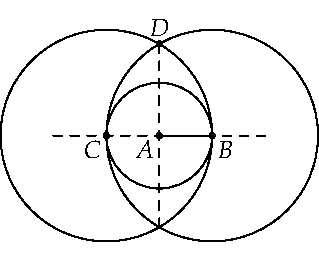
\includegraphics{euclid-I11}
				&
				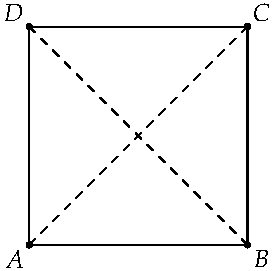
\includegraphics{euclid-I46}
				&
				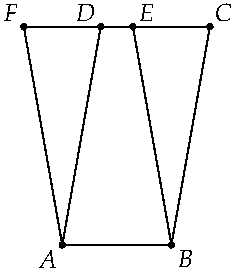
\includegraphics{euclid-I35a}
				\\[-2pt]
				Theorem I.\,11
				&
				Theorem I.\,46
				&
				Theorem I.\,35
			\end{tabular}
		\end{center}
		
	  
	  \item Consider spherical geometry (page \pageref{pg:sphere}), where \emph{lines} are paths of shortest distance (great circles).
	 	\begin{enumerate}
	 	  \item Which of Euclid's postulates P1--P5 are satisfied by this geometry?
	  	\item (Hard)\lstsp Where does the proof of the exterior angle theorem \emph{fail} in spherical geometry? 
	 	\end{enumerate}
	  
	  
	  \item\begin{enumerate}
	    \item State the negation of Playfair's postulate.
	    \item Prove that Playfair's postulate is equivalent to the following statement:
	  \begin{quote}
	  	Whenever a line is perpendicular to one of two parallel lines, it must be perpendicular to the other.
	  \end{quote}
	  \end{enumerate}
	 
	  
	  \item\label{ex:euclidundecideable} The \emph{line-circle continuity} property states:
	  \begin{quote}
	  If point $P$ lies inside and $Q$ lies outside a circle $\alpha$, then the segment $\overline{PQ}$ intersects $\alpha$.
	  \end{quote}
	  By considering the set of rational points in the plane $\Q^2=\{(x,y):x,y\in\Q\}$, and making a sensible definition of line and circle, show that the line-circle continuity property is undecidable within Euclid's system.
		
		
		\item The standard proof of the converse of Pythagoras' theorem (I.\,48) is, in fact, a \emph{corollary} of Pythagoras' Theorem! Look it up and explain it as best you can.
	\end{enumerate}
	
\end{exercises}

\clearpage



\subsection{Hilbert's Axioms, part I: Incidence and Order}\label{sec:hilbert1}

The \emph{Elements} contains several errors and omissions. Over the centuries, mathematicians identified and attempted to correct these. The culmination of this work came with the publication of David Hilbert's \emph{Grundlagen der Geometrie (Foundations of Geometry)} in 1899.\smallbreak

%This was followed by George Birkhoff's axiomatization of Analytic Geometry (geometry with co-ordinates) in 1932.

Hilbert's axioms for plane geometry\footnote{Hilbert also treated 3D geometry; we only give the axioms relevant to plane geometry. The axioms are almost perfect with regard to our desired properties. There is essentially only one model (standard Cartesian geometry); this is almost but not quite the same as completeness. In the absence of the continuity axiom, they are consistent; in line with Gödel, consistency cannot be proved once continuity is included. As stated, the axioms are not quite independent: O-3 does not require existence (follows from Pasch's axiom), C-1 does not require uniqueness (follows from uniqueness in C-4) and C-6 can be weakened. Hilbert's axioms were revised after publication; we've only stated one version.} are listed on the next page. We use his system to explore some of the problems in Euclid and how they may be addressed.\smallbreak


Hilbert's undefined terms consist of two types of object (\emph{points} and \emph{lines}), and three relations (\emph{between $*$, on $\in$} and \emph{congruence $\cong$}). For brevity we'll often (ab)use set notation, essentially viewing a line as a set of points, though this is not necessary. At various places, definitions and notations are required.

\begin{defn}{}{hilbertbasic}
	Throughout, $A,B,C$ denote points and $\ell,m$ lines.
	\begin{description}\itemsep 0pt plus 1pt
	  \item[\normalfont\emph{Line}:] $\smash[t]{\lin{AB}}$ denotes the line through distinct $A,B$. This exists and is unique by axioms I-1 and I-2.
	  \item[\normalfont\emph{Segment}:] $\cl{AB}=\{A,B\}\cup\{C:A*C*B\}$ consists of distinct \emph{endpoints} $A,B$ and all \emph{interior} points $C$ lying between them.
	  \item[\normalfont\emph{Ray}:] $\ray{AB}=\cl{AB}\cup\{C:A*B*C\}$ is a ray with \emph{vertex} $A$. In essence, we extend $\cl{AB}$ beyond $B$.
	  \item[\normalfont\emph{Triangle}:] $\triangle ABC=\cl{AB}\cup\cl{BC}\cup\cl{CA}$ where $A,B,C$ are non-collinear. Triangles are \emph{congruent} if their sides and angles are congruent in pairs.
		\item[\normalfont\emph{Sidedness}:] Distinct $A,B$ (not on $\ell$) lie on the \emph{same side} of $\ell$ if $\cl{AB}\cap\ell=\emptyset$. Otherwise $A$ and $B$ lie on \emph{opposite sides} of $\ell$.
		\item[\normalfont\emph{Angle}:] $\angle BAC=\ray{AB}\cup\ray{AC}$ has \emph{vertex} $A$ and \emph{sides} $\ray{AB}$ and $\ray{AC}$.
		\item[\normalfont\emph{Parallelism}:] Lines $\ell$ and $m$ \emph{intersect} if there exists a point lying on both: $\exists A\in\ell\cap m$. Lines are \emph{parallel} if they do not intersect. Segments/rays are parallel if the corresponding lines are parallel.
	\end{description}
	The pictures represent these notions in the usual model of Cartesian geometry.
	\begin{center}
		\begin{tabular}{@{}c@{\qquad}c@{\qquad}c@{\qquad}c@{}}
			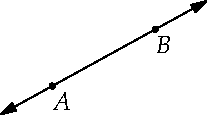
\includegraphics{hilbert-def-line}
			&
			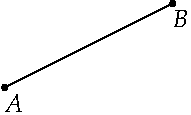
\includegraphics{hilbert-def-seg}
			&
			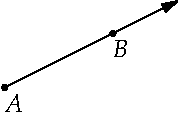
\includegraphics{hilbert-def-ray}
			&
			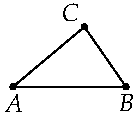
\includegraphics{hilbert-def-triangle}
			\\
			Line $\lin{AB}$
			&
			Segment $\cl{AB}$
			&
			Ray $\ray{AB}$
			&
			Triangle $\triangle ABC$
			\\[12pt]
			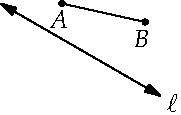
\includegraphics{hilbert-def-side}
			&
			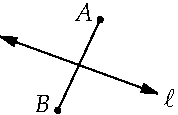
\includegraphics{hilbert-def-side2}
			&
			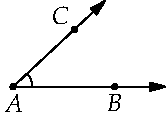
\includegraphics{hilbert-def-angle}
			&
			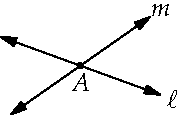
\includegraphics{hilbert-def-intersect}
			\\
			Same side
			&
			Opposite sides
			&
			Angle $\angle BAC$
			&
			Intersection $A\in\ell\cap m$
		\end{tabular}
	\end{center}
\end{defn}


\pagebreak
\thispagestyle{empty}
\begin{center}
\bfseries\Large Hilbert's Axioms for Plane Geometry
\end{center}

\begin{minipage}[t]{0.46\linewidth}
\boldinline{Undefined terms}
\begin{enumerate}\itemsep2pt
  \item \emph{Points}: \ use capital letters, $A,B,C\ldots$
  \item \emph{Lines}: \ use lower case letters, $\ell,m,n,\ldots$
  \item \emph{On}: \ $A\in\ell$ is read `$A$ lies on $\ell$'
  \item \emph{Between}: \ $A*B*C$ is read `$B$ lies between $A$ and $C$'
  \item \emph{Congruence}: \ $\cong$ is a binary relation on segments or angles
\end{enumerate}

\boldinline{Axioms of Incidence}

\begin{enumerate}
	\item[I-1] For any distinct $A,B$ there exists a line $\ell$ on which lie $A,B$.
	\item[I-2] There is at most one line through distinct $A,B$ \ ($A$ and $B$ both \emph{on} the line).
\end{enumerate}\vspace{-2pt}
	
Notation: \emph{line} $\overleftrightarrow{AB}$ through $A$ and $B$\vspace{-2pt}

\begin{enumerate}\setcounter{enumi}{2}	
	\item[I-3] On every line there exist at least two distinct points. There exist at least three points not all on the same line.
\end{enumerate}


\boldinline{Axioms of Order}

\begin{enumerate}
	\item[O-1] If $A*B*C$, then $A,B,C$ are distinct points on the same line and $C*B*A$.
	\item[O-2] Given distinct $A,B$, there is at least one point $C$ such that $A*B*C$.
	\item[O-3] If $A,B,C$ are distinct points on the same line, exactly one lies between the others.
\end{enumerate}\vspace{-2pt}
	
Definitions: \emph{segment} $\cl{AB}$ and \emph{triangle} $\triangle ABC$\vspace{-2pt}

\begin{enumerate}\setcounter{enumi}{3}	
	\item[O-4] (Pasch's Axiom) Let $\triangle ABC$ be a triangle and $\ell$ a line not containing any of $A,B,C$. If $\ell$ contains a point of the segment $\cl{AB}$, then it also contains a point of either $\cl{AC}$ or $\cl{BC}$. 
\end{enumerate}

Definitions: \emph{sides} of line $\overleftrightarrow{AB}$ and \emph{ray} $\ray{AB}$
\end{minipage}
\hfill
\begin{minipage}[t]{0.48\linewidth}
\boldinline{Axioms of Congruence}

\begin{enumerate}
  \item[C-1] (Segment transference) \ Let $A,B$ be distinct and $r$ a ray based at $A'$. Then there exists a unique point $B'\in r$ for which $\cl{AB}\cong\cl{A'B'}$. Moreover $\cl{AB}\cong\cl{BA}$.
  \item[C-2] If $\cl{AB}\cong\cl{EF}$ and $\cl{CD}\cong\cl{EF}$, then $\cl{AB}\cong\cl{CD}$.
  \item[C-3] If $A*B*C$, \ $A'*B'*C'$, \ $\cl{AB}\cong\cl{A'B'}$ and $\cl{BC}\cong\cl{B'C'}$, then $\cl{AC}\cong\cl{A'C'}$.
  \end{enumerate}
	
Definitions: \emph{angle} $\angle ABC$\vspace{-2pt}

\begin{enumerate}\setcounter{enumi}{3}
  \item[C-4] (Angle transference) \ Given $\angle BAC$ and $\ray{A'B'}$, there exists a unique ray $\ray{A'C'}$ on a given side of $\overleftrightarrow{A'B'}$ for which $\angle BAC\cong\angle B'A'C'$.
  \item[C-5] If $\angle ABC\cong\angle GHI$ and $\angle DEF\cong\angle GHI$, then $\angle ABC\cong\angle DEF$. Moreover, $\angle ABC\cong\angle CBA$.
  \item[C-6] (Side-angle-side) Given triangles $\triangle ABC$ and $\triangle A'B'C'$, if $\cl{AB}\cong\cl{A'B'}$, $\cl{AC}\cong\cl{A'C'}$, and $\angle BAC\cong\angle B'A'C'$, then the triangles are congruent.\footnotemark{}
\end{enumerate}

\boldinline{Axiom of Continuity}\phantom{bob}\smallbreak

Suppose $\ell$ is partitioned into non-empty subsets $\Sigma_1,\Sigma_2$ such that no point of $\Sigma_1$ lies between two points of $\Sigma_2$ and vice versa.\par
Then there exists a unique point $\mathcal O\in\ell$ satisfying $P_1*\mathcal O*P_2$, if and only if $\mathcal O\neq P_1$, $\mathcal O\neq P_2$ and one of $P_1$ or $P_2$ lies in $\Sigma_1$ and the other in $\Sigma_2$.\medbreak



\boldinline{Playfair's Axiom}\phantom{bob}\smallbreak

Definition: \emph{parallel lines}\smallbreak

Given a line $\ell$ and a point $P$ not on $\ell$, there exists at most one line through $P$ parallel to $\ell$.
\end{minipage}

\footnotetext{Its sides/angles are congruent in pairs. We extend congruence to other geometric objects similarly.}

\clearpage





\boldsubsubsection{Axioms of Incidence: Finite Geometries}

The axioms of incidence describe the relation \emph{on.} An \emph{incidence geometry} is any model satisfying the axioms I-1, I-2, I-3. Perhaps surprisingly, there exist geometries with \emph{finitely many points}!

\begin{examples}{}{fano}
	By I-3, an incidence geometry requires \emph{at least three} points.\par
	\begin{minipage}[t]{0.62\linewidth}\vspace{-5pt}
		A 3-point geometry exists, and is unique up to relabelling:\smallbreak
		I-3 says the points $A,B,C$ must be non-collinear. By I-1 and I-2, each pair lies on a unique line, whence there are precisely three lines
		\[
			\ell=\{A,B\},\quad m=\{A,C\},\quad n=\{B,C\}
		\]
		Up to relabelling, there are two incidence geometries with four points: one is drawn; how many lines has the other?
	\end{minipage}
	\hfill
	\begin{minipage}[t]{0.37\linewidth}\vspace{-15pt}
		\flushright
		\begin{tabular}{cc@{}}
			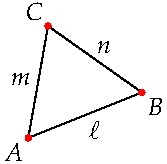
\includegraphics{hilbert-incidence3}
			&
			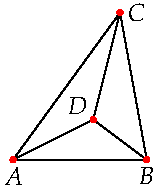
\includegraphics{hilbert-incidence4}\\
			3 points, 3 lines
			&
			%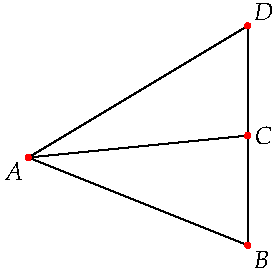
\includegraphics{hilbert-incidence4-2}
			4 points, 6 lines%&4 points, 4 lines
		\end{tabular}
	\end{minipage}
	\smallbreak
	\begin{minipage}[t]{0.72\linewidth}\vspace{0pt}
		The final picture is a famous example known as the \emph{Fano plane,} an incidence geometry with seven points and seven lines which finds applications in many places, including combinatorics. Each point lies on precisely three lines; each dot is colored to indicate the lines to which it belongs. Don't be fooled by the black line looking curved and seeming to cross the blue line near the top; it really only contains three points!
	\end{minipage}
	\hfill
	\begin{minipage}[t]{0.27\linewidth}\vspace{-17pt}
		\flushright
		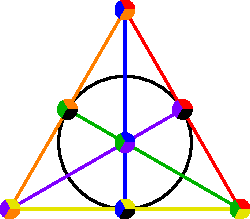
\includegraphics{hilbert-incidence7}
	\end{minipage}
\end{examples}

We can even prove some simple theorems in incidence geometry.

\begin{lemm}{}{intersectunique}
	If distinct lines intersect, then they do so in exactly one point.
\end{lemm}

\begin{proof}
	Suppose $A,B$ are distinct points of intersection. By axiom I-2, there is exactly one line through $A$ and $B$. Contradiction.
\end{proof}

\begin{lemm}{}{incidenceeasy}
	Through any point there exists at least two lines.
\end{lemm}

The proof is an exercise. While incidence geometry is fun, our main goal is to understand Euclidean geometry, so we move on to the next set of axioms.


\boldsubsubsection{Axioms of Order: Sides of a Line and Pasch's Axiom}

The axioms of order describe the ternary relation \emph{between.} Their inclusion in Hilbert's axioms is due in no small part to the work of Moritz Pasch, after whom Pasch's axiom (O-4, c.\,1882) is named. Pasch's axiom is very powerful; in particular, it permits us to define the \emph{interiors} of several geometric objects, and to see that these are non-empty.

\begin{lemm}{}{seginterior}
	Every segment contains an interior point.
\end{lemm}

We leave the proof to Exercise \ref{exs:seginterior}. By inducting on the Lemma, every segment contains \emph{infinitely many} points, whence the above finite geometries are not valid models once the order axioms are included.

\goodbreak

To get much further, it is necessary to establish that a line has precisely two \emph{sides} (Definition \ref{defn:hilbertbasic}). This concept lies behind several of Euclid's arguments, without being properly defined in the \emph{Elements.}


\begin{thm}{Plane Separation}{planesep}
	A line $\ell$ separates all points not on $\ell$ into two half-planes; the two \emph{sides} of $\ell$. Explicitly: suppose none of the points $A,B,C$ lie on $\ell$, then:
	\begin{enumerate}\itemsep0pt
	  \item If $A,B$ lie on the same side of $\ell$ and $B,C$ lie on the same side, then $A,C$ lie on the same side.
	  \item If $A,B$ lie on opposite sides and $B,C$ lie on opposite sides, then $A,C$ lie on the same side.
	  \item If $A,B$ lie on opposite sides and $B,C$ lie on the same side, then $A,C$ lie on opposite sides.
	\end{enumerate}\vspace{-10pt}
	\begin{center}
		\begin{tabular}{c@{\qquad}c@{\qquad}c}
			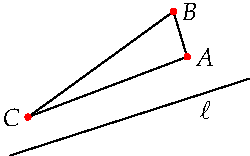
\includegraphics{hilbert-planesep}
			&
			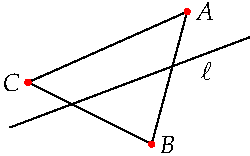
\includegraphics{hilbert-planesep2}
			&
			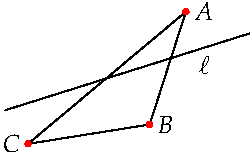
\includegraphics{hilbert-planesep3}
			\\
			Case 1
			&
			Case 2
			&
			Case 3
		\end{tabular}
	\end{center}
\end{thm}

\begin{proof}
Suppose $A,B,C$ are non-collinear. If $\cl{AC}$ intersects $\ell$, then $\ell$ intersects one of the sides of $\triangle ABC$. By Pasch's axiom, it also intersects either $\cl{AB}$ or $\cl{BC}$. This is the contrapositive of case 1.\smallbreak
The other cases are exercises, and we omit the tedious collinear possibilities.
\end{proof}

Plane separation and its attendant half-planes allow us to properly define the interiors of angles and triangles. 

\begin{defn}{}{interiorangle}
	A point $I$ is \emph{interior} to angle $\angle BAC$ if:\par
	\begin{minipage}[t]{0.7\linewidth}\vspace{-3pt}
	\begin{itemize}%\itemsep0pt
	  \item $I$ lies on the same side of $\lin{AB}$ as $C$, and,
	  \item $I$ lies on the same side of $\lin{AC}$ as $B$.
	\end{itemize}
	Otherwise said, $I$ lies in the intersection of two half-planes.
	\end{minipage}
	\hfill
	\begin{minipage}[t]{0.29\linewidth}\vspace{-12pt}
		\flushright
		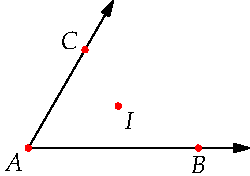
\includegraphics{hilbert-interior}
	\end{minipage}
	\bigbreak
	A point $I$ is \emph{interior} to a triangle $\triangle ABC$ if it lies in the intersection of three of the half-planes defined by the edges of the triangle. Equivalently, it is interior to all three of the angles $\angle ABC$, $\angle BAC$ and $\angle ACB$.
\end{defn}

Interior points permit us to compare angles: if $I$ is interior to $\angle BAC$, then $\angle BAI<\angle BAC$ has obvious meaning, \emph{without resorting to numerical angle measure.}

\begin{cor}{}{angleinteriorexist}
	Every angle has an interior point.
\end{cor}

\begin{proof}
	Given $\angle BAC$, consider any interior point $I$ of the segment $\cl{BC}$. This plainly lies on the same side of $\lin{AB}$ as $C$ and on the same side of $\lin{AC}$ as $B$.
\end{proof}

In Exercise \ref{exs:seginfinite}, we check that the interior of a triangle is non-empty.

\goodbreak

Pasch's axiom could be paraphrased as follows: \emph{If a line enters a triangle, it must come out.} We haven't quite established this crucial fact however. What if the line passes through a vertex?
 
\begin{thm}[lower separated=false, sidebyside, sidebyside align=top seam, sidebyside gap=0pt, righthand width=0.3\linewidth]{Crossbar Theorem}{}
	Suppose $I$ is interior to $\angle BAC$. Then $\ray{AI}$ intersects $\cl{BC}$.\medbreak
As a special case; if a line passes through a vertex and an interior point of a triangle, then it intersects the side opposite the vertex.
	\tcblower
	\flushright
	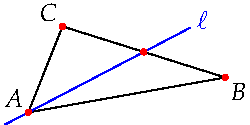
\includegraphics{hilbert-pasch2}
\end{thm}


\begin{proof}
	Extend $\cl{AB}$ to a point $D$ such that $A$ lies between $B$ and $D$ (O-2). Since $C$ is not on $\lin{BD}=\lin{AB}$ we have a triangle $\triangle BCD$. Since $\lin{AI}$ intersects one edge of $\triangle BCD$ at $A$ and does not cross any vertices, Pasch says it intersects one of the other edges ($\cl{BC}$ or $\cl{CD}$) at a point $M$.
	\begin{itemize}
	  \item If $I=M\in\cl{BC}$, we're done. 
	 	\item If $I=M\in\cl{CD}$, a contradiction follows from Exercise \ref{exs:bernays} and plane separation.
	\end{itemize}
	Otherwise, if $I\neq M$, observe:
	%The point $A$ is therefore the unique intersection of three distinct lines: $\lin{AB}$, $\lin{AC}$ and $\lin{IM}$. Moreover:
	\begin{itemize}
	  \item Since $I$ is interior to $\angle BAC$, it lies on the same side of $\smash[t]{\lin{AB}=\lin{BD}}$ as $C$.
	  \item Since $M\in\cl{BC}\cup\cl{CD}$, it lies on the same side of $\smash[t]{\lin{AB}=\lin{BD}}$ as $C$.
	\end{itemize}
	By the plane separation theorem, $I$ and $M$ lie on the \emph{same side} of $\smash[t]{\lin{AB}}$. In particular,
	\[
		A\not\in\smash[t]{\cl{IM}}\implies M\in\smash[t]{\ray{AI}}
	\]
	The two generic cases are drawn below (these encompass arrangements where $I$ lies \emph{inside} $\triangle ABC$); it suffices to show that the second case is impossible.
	\begin{center}
		\begin{tabular}{cc}
			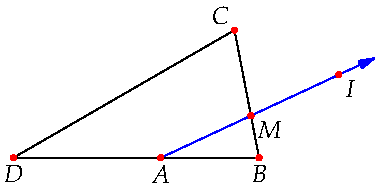
\includegraphics[scale=0.95]{hilbert-crossbar1}&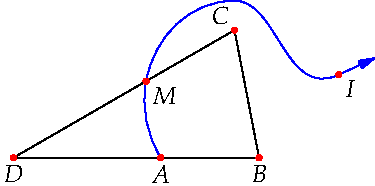
\includegraphics[scale=0.95]{hilbert-crossbar2}%\\
			%correct arrangement&impossible case
		\end{tabular}
	\end{center}
	If $M\in\cl{CD}$, then $I$ and $M$ are on \emph{opposite sides} of $\lin{AC}$. But then $\cl{IM}$ intersects $\lin{AC}$, which it must do at $A$. This contradicts the fact that $A\not\in\cl{IM}$.
\end{proof}



\begin{minipage}[t]{0.67\linewidth}\vspace{-3pt}
	Euclid repeatedly uses the crossbar theorem without justification, including in his construction of perpendiculars and of angle and segment bisectors (Theorems I.\,9+10); we sketch this here.\smallbreak
	Given $\angle BAC$, construct $E$ such that $\cl{AB}\cong\cl{AE}$. Construct $D$ using an equilateral triangle (I.\,1). SSS (I.\,8) shows that the angle is bisected, and SAS (I.\,4) that $\ray{AD}$ bisects $\cl{BE}$.\smallbreak
	Unfortunately Euclid gives no argument for why $D$ is interior to $\angle BAC$ or why $\ray{AD}$ should intersect $\cl{BE}$!
\end{minipage}
\hfill
\begin{minipage}[t]{0.32\linewidth}\vspace{0pt}
	\flushright
	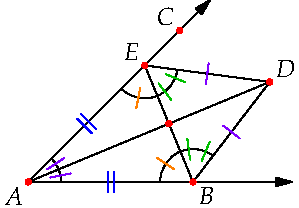
\includegraphics{hilbert-bisect}
\end{minipage}
\medbreak


Even with Pasch's axiom and the crossbar theorem, it requires some effort to repair Euclid's proof. No matter, we'll provide an alternative construction of the bisector once we've considered congruence.

\goodbreak


\begin{exercises}
	\exstart Label the vertices in the Fano plane 1 through 7 (any way you like). As we did in Example \ref{ex:fano} for the 3-point geometry, describe each line in terms of its points.
	\begin{enumerate}\setcounter{enumi}{1}
	  \item Prove Lemma \ref{lemm:incidenceeasy}.
	  
	  
	  \item Give a model for each of the 5-point incidence geometries: how many are there?\par
	  (\emph{Hint: remember that order doesn't matter, so the only issue is how many points lie on each line})
	  
	    
	  \item Consider the proof of the crossbar theorem. Explain how we know that $\smash[t]{\ray{AI}}$ does not contain any of the vertices of $\triangle BCD$.
	  
	  
	  \item\label{exs:seginterior} You are given distinct points $A,B$. Using the axioms of incidence and order and Lemma \ref{lemm:intersectunique} (follows from I-2), show the existence of each of the points $C,D,E,F$ in the picture \emph{in alphabetical order.} Hence conclude the existence of a point $F$ lying \emph{between} $A$ and $B$ (Lemma \ref{lemm:seginterior}).\par
	  \begin{minipage}[t]{0.65\linewidth}\vspace{-5pt}
	  During your construction, address the following issues:
	  \begin{enumerate}\itemsep0pt
	    \item Explain why $D$ does not lie on $\overleftrightarrow{AB}$.
			\item Explain why $E$ does not lie on $\triangle ABD$.
			\item Explain why $E\neq C$ (whence $\overleftrightarrow{CE}$ exists).
			\item Explain why $F$ lies on $\cl{AB}$ and \emph{not} on $\cl{BD}$.
		\end{enumerate}
	  \end{minipage}
	  \hfill
	  \begin{minipage}[t]{0.34\linewidth}\vspace{-5pt}
	  	\flushright
	  	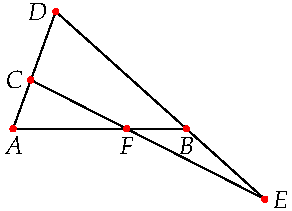
\includegraphics[scale=0.9]{hilbert-between}
	  \end{minipage}
	  
	  
	  \item\label{exs:bernays} We complete the proof of the plane separation theorem (\ref{thm:planesep}).
	  \begin{enumerate}
	    \item Prove part 3 (it is almost a verbatim application of Pasch's axiom).\par
	    \begin{minipage}[t]{0.75\linewidth}\vspace{-5pt}
	    \item Suppose a line $\ell$ intersects all three sides of $\triangle ABC$ but no vertices. This results in a very strange picture: we've labelled the intersections $D,E,F$ and WLOG chosen $D*E*F$.\smallbreak
	    Apply Pasch's axiom to $\triangle DBF$ and $\lin{AC}$ to obtain a contradiction. Hence establish part 2 of the plane separation theorem.    
	    \end{minipage}
	    \hfill
	    \begin{minipage}[t]{0.24\linewidth}\vspace{-25pt}
	    	\flushright
	    	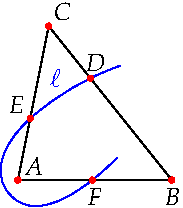
\includegraphics{hilbert-bernays}
	    \end{minipage}
	  \end{enumerate}
	  
	  
	  \item Suppose $A,B,C$ are distinct points on a line $\ell$.
	  \begin{enumerate}
	    \item Explain why there exists a line $m\neq \ell$ such that $B\in m$.
	    \item Prove that $A*B*C\iff A$ and $C$ lie on opposite sides of $m$.
	    \item Suppose $A*B*C$. Use part (b) to prove the following:
	    \begin{enumerate}
				\item $B$ is the only point common to the rays $\ray{BA}$ and $\ray{BC}$.
				\item If $D\in\ell$ is any point other than $B$, prove that $D$ lies in precisely one of $\ray{BA}$ or $\ray{BC}$.
			\end{enumerate}
	  \end{enumerate}
	  
	  
	  \item\label{exs:seginfinite} Prove that the interior of a triangle is non-empty.\par
	  (\emph{Hint: use Exercise \ref{exs:seginterior} to construct a suitable $I$, then prove that it lies on the correct side of each edge})
	  
	\end{enumerate}
\end{exercises}


\clearpage



\subsection{Hilbert's Axioms, part II: Congruence}\label{sec:hilbert2}

The congruence axioms formalize Euclid's constructions and pictorial reasoning, and replace his confusing use of \emph{equal.} Segments/angles are now equal only when they are exactly the same; this is the \emph{reflexivity} part of the following, which depends only on axioms C-1, C-2, C-4 and C-5.

\begin{lemm}{}{}
Congruence of segments/angles is an equivalence relation.
\end{lemm}

% \begin{proof}
% 	\begin{description}\itemsep0pt
%   	\item[Reflexivity]\quad Let $\cl{AB}$ be given and apply C-1 to obtain a segment %\footnote{You could even take $A'=A$ and use the ray $r=\ray{AB}$!}
%   	 $\cl{A'B'}$ such that $\cl{AB}\cong\cl{A'B'}$. We sneakily use this \emph{twice} and apply C-2:
%   	\[\cl{AB}\cong\cl{A'B'}\text{ and } \cl{AB}\cong\cl{A'B'}\implies \cl{AB}\cong\cl{AB}\]
%   	\item[Symmetry]\quad Assume $\cl{AB}\cong\cl{CD}$. By reflexivity, $\cl{CD}\cong\cl{CD}$. By C-2 we have $\cl{CD}\cong\cl{AB}$.
%   	\item[Transitivity]\quad If $\cl{AB}\cong\cl{CD}$ and $\cl{CD}\cong\cl{EF}$, apply symmetry  and C-2 to conclude $\cl{AB}\cong\cl{EF}$.\\[-5pt]
%   \end{description}
%   Axioms C-4 and C-5 say essentially the same thing for angles.
% \end{proof}

\boldinline{Segment/Angle Transfer and Comparison}

Neither Hilbert nor Euclid require an \emph{absolute} notion of length, though both require a method for \emph{comparing} lengths. 


\begin{defn}[lower separated=false, sidebyside, sidebyside align=top seam, sidebyside gap=0pt, righthand width=0.35\linewidth]{}{lengthcomp}
Let segments $\cl{AB}$ and $\cl{CD}$ be given.\smallbreak
Using axiom C-1, construct the unique point $E$ on $\ray{CD}$ such that $\cl{CE}\cong\cl{AB}$: we have now \emph{transferred} $\cl{AB}$ onto $\ray{CD}$.\smallbreak
We write $\cl{AB}<\cl{CD}$ if $E$ lies between $C$ and $D$, etc.
\tcblower
\flushright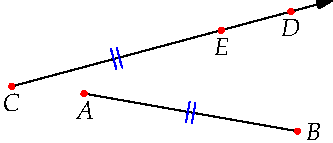
\includegraphics[scale=0.95]{angles-compare}
\end{defn}

By O-3, any segments are comparable: given $\cl{AB}$, $\cl{CD}$, precisely one of the following holds,
\[\cl{AB}<\cl{CD},\qquad \cl{CD}<\cl{AB},\qquad\cl{AB}\cong\cl{CD}\]
C-3 says that congruence respects the addition of congruent segments. Unique angle transfer, comparison and addition follow similarly from axiom C-4 and Definition \ref{defn:interiorangle} (interior points).


\boldinline{Side-Angle Side (SAS)}

Euclid `proves' SAS (I.\,4) by the unjustified procedure of laying one triangle on top of another. It was ultimately realized that at least one triangle congruence (SAS, ASA, SSS and SAA) had to be an axiom. Hilbert assumes\footnote{Hilbert in fact assumed a weaker version; see Exercise \ref{exs:hilbertsas}.}
SAS and proceeds to prove the remainder. For example:

\begin{thm}{Angle-Side-Angle/ASA, Euclid I.\,26, case I}{asa}
Suppose $\triangle ABC$ and $\triangle DEF$ satisfy
\[\angle ABC\cong\angle DEF,\qquad \cl{AB}\cong\cl{DE},\qquad\angle BAC\cong\angle EDF\]
Then the triangles are congruent \ ($\angle ACB\cong\angle DFE$, \ $\cl{AC}\cong\cl{DF}$ and $\cl{BC}\cong\cl{EF}$).
\end{thm}

Remember that we don't yet have uniqueness of parallels, so we can't assume $\angle ACB\cong\angle DFE$!

\begin{proof}
Segment transfer provides the unique point $G\in \ray{EF}$ such that \textcolor{orange}{$\cl{EG}\cong \cl{BC}$}.\par
\begin{minipage}[t]{0.65\linewidth}\vspace{0pt}
SAS says \textcolor{red}{$\angle EDG\cong\angle BAC\cong \angle EDF$} (the last by assumption).\medbreak
Since $F$ and $G$ lie on the same side of $\lin{DE}$, angle transfer (C-4) says that they lie on the \emph{same ray} through $D$.\medbreak
But then $F$ and $G$ both lie on two distinct lines ($\lin{EF}$ and $\lin{DF}$): we conclude that $F=G$.\medbreak
By SAS we conclude that $\triangle ABC\cong\triangle DEF$.
\end{minipage}
\begin{minipage}[t]{0.34\linewidth}\vspace{-28pt}
\flushright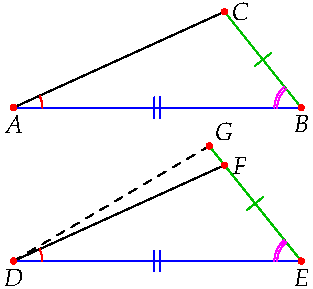
\includegraphics[scale=0.95]{angles-asa}
\end{minipage}
\end{proof}


\goodbreak


\boldsubsubsection{Geometry Without Circles}

Circles are at the heart of Euclid's constructions---his very first result depends on them! Yet, for reasons we'll deal with shortly, Hilbert essentially ignores circles. We sketch a few of his alternative approaches to Euclid's basic results.

\begin{thm}{Euclid I.\,5}{euclidiso}
An isosceles triangle has congruent base angles.
\end{thm}

Isosceles means \emph{equal legs}: two sides of the triangle are congruent. The remaining side is the \emph{base.}\smallbreak
Euclid's argument relies on a famously complicated construction (look it up!). Hilbert does things more speedily.

\begin{tcolorbox}[proofstyle]
\begin{minipage}[t]{0.7\linewidth}\vspace{0pt}
\emph{Proof.}\lstsp Suppose that $\triangle ABC$ is isosceles where $\cl{AB}\cong\cl{AC}$. Consider a `new' triangle $\triangle A'B'C'=\triangle ACB$ where the base points are switched:
\[A'=A,\qquad B'=C,\qquad C'=B\]
We have:
\begin{itemize}
  \item $\angle BAC\cong\angle CAB$ (C-5) $\implies\angle BAC\cong\angle B'A'C'$.
  \item $\cl{AB}\cong\cl{AC}\implies \cl{AB}\cong\cl{A'B'}$ and $\cl{AC}\cong\cl{A'C'}$.
\end{itemize}
SAS says that $\angle ABC\cong\angle A'B'C'\cong\angle ACB$.
\end{minipage}\hfill\begin{minipage}[t]{0.29\linewidth}\vspace{0pt}
\flushright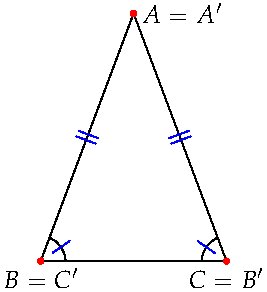
\includegraphics{angles-isos2}\\[-8pt]
\hfill\qedsymbol
\end{minipage}
\end{tcolorbox}


The proof is very sneaky; Hilbert simply relabels the original triangle and applies SAS! The converse to this statement follows from the ASA congruence (Exercise \ref{exs:isoconverse}).\bigbreak



\begin{minipage}[t]{0.7\linewidth}\vspace{0pt}
\boldinline{Dropping a Perpendicular}

Suppose $C$ does not lie on $\ell$. By axiom I-3, $\ell=\lin{AB}$ for some points $A,B$.\smallbreak
Use axioms C-4 and C-1 to transfer \textcolor{Green}{$\angle BAC$} to the other side of the line at $A$, creating a new point $D$.\smallbreak
Since $C$ and $D$ lie on opposite sides of $\lin{AB}$, it must intersect $\cl{CD}$ at some point $M$.\smallbreak
SAS applied to $\triangle MAC$ and $\triangle MAD$ shows that $\angle AMC\cong\angle AMD$: since these sum to a straight edge, they must be right-angles.
\begin{itemize}\itemsep0pt
  \item The construction still works if \textcolor{Green}{$\angle BAC$} is greater than a right-angle: $\angle MAC$ is now supplementary to $\angle BAC$ rather than equal.
  \item In the extreme case $M=A$, we have no triangles and SAS cannot be applied. Instead follow the same argument starting with $\angle ABC$.
\end{itemize}
\end{minipage}\begin{minipage}[t]{0.3\linewidth}\vspace{0pt}
\flushright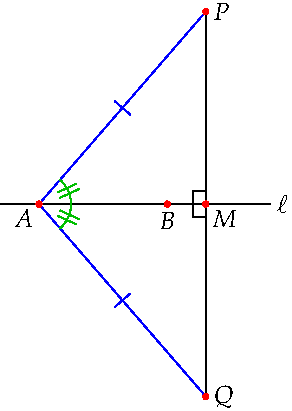
\includegraphics{angles-perp}
\end{minipage}\bigbreak

A generalization of this construction facilitates a corrected argument for the SSS congruence: Euclid again resorted to his flawed `laying on top of' reasoning.

\begin{thm}{Side-Side-Side/SSS, Euclid I.\,8}{}
If triangles have sides congruent in pairs, then the triangles are congruent.
\end{thm}


\begin{tcolorbox}[proofstyle, lower separated=false, sidebyside, sidebyside align=top seam, sidebyside gap=0pt, righthand width=0.4\linewidth]
\emph{Proof.}\lstsp Suppose $\triangle ABC$ and $\triangle DEF$ have sides congruent in pairs as shown.\smallbreak
Transfer \textcolor{orange}{$\angle EDF$} to $A$ on the other side of $\cl{AB}$ from $C$ to obtain $G$ (axioms C-4 and C-1).\smallbreak
SAS shows that $\triangle BAG\cong\triangle EDF$ and so $\textcolor{orange}{\cl{BG}\cong\cl{EF}\cong\cl{BC}}$.\smallbreak
Joining $\cl{CG}$ produces two isosceles triangles $\triangle ACG$ and $\triangle BCG$ with base $\cl{CG}$. Both have and congruent base angles at $C$ and $G$.\smallbreak
Summing angles at $C$ and $G$ and applying SAS shows that $\triangle ACB\cong\triangle AGB\cong\triangle DFE$ as required.\medbreak
As with the perpendicular argument previously, we should also carefully deal with the situations where the sum is a subtraction or the triangle is right-angled at $A$ or $B$.
\tcblower
\flushright\includegraphics{angles-sss}\\[-10pt]\hfill\qedsymbol
\end{tcolorbox}

\boldinline{Exterior Angle Theorem (\ref{thm:extangle}) (Euclid I.\,16)}

Euclid's approach requires a bisector which he obtains from circles. Hilbert does things a little differently.

\begin{proof}
Given $\triangle ABC$, extend $\cl{AB}$ to $D$ such that \textcolor{blue}{$\cl{AC}\cong\cl{BD}$}.\smallbreak
In the first picture below, assume\ \textcolor{Green}{$\delta\cong\gamma$}. Apply SAS to see that $\triangle ACB\cong\triangle DBC$: in particular \textcolor{blue}{$\epsilon\cong\beta$}.\smallbreak
Clearly $A$ and $D$ lie on opposite sides of $\lin{BC}$: but then $\epsilon+\gamma\cong \beta+\delta$ is a straight edge and so $A,D$ are distinct points lying on \emph{two} lines! Contradiction.\smallbreak
We conclude that $\delta\ncong\gamma$.
\begin{center}
\begin{tabular}{c@{\qquad}c}
\includegraphics[scale=0.95]{angles-exterior1}&\includegraphics[scale=0.95]{angles-exterior2}\\
Step 1: $\delta\cong\gamma$ is a contradiction&Step 2: $\delta<\gamma$ is a contradiction
\end{tabular}
\end{center}
In the second picture, assume $\delta<\gamma$. Transfer the angle to $C$ as shown where $\eta\cong\delta$: by the crossbar theorem, we obtain an intersection point $E$. But now $\delta$ is an exterior angle of $\triangle EBC$ which is congruent to an interior angle $\eta$ of the same triangle: contradiction.\smallbreak
The only non-contradictory possibility is that $\delta>\gamma$.\smallbreak
By taking the vertical angle to $\delta$ at $B$ and repeating the argument, we also see that $\delta>\alpha$.
\end{proof}

The exterior angle theorem also proves that the sum of any two angles in a triangle is strictly less than a straight edge: $\alpha+\beta<\delta+\beta =\ang{180}$.

\goodbreak

\boldinline{Is Euclid now fixed?}

Almost! In the exercises we show how the following may be achieved in Hilbert's system:
\begin{itemize}
  \item Construction of an isosceles triangle on a segment $\cl{AB}$. With this one can construct segment and angle bisectors (Euclid I.\,9+10).
  \item SAA congruence (Euclid I.\,26, case II): the last remaining triangle congruence theorem.
\end{itemize}

At this point we've recovered almost all of Book I prior to the application of the parallel postulate. Including Playfair's axiom allows the remainder of Book I to be completed, including Pythagoras', all \emph{without circles!}

\begin{exercises}
Except for questions \ref*{exs:aaassano} and \ref*{ex:pythagnocont}, all exercises should be answered in \emph{neutral geometry,} with no reference to the continuity axiom, circles, or anything regarding uniqueness of parallels such as Playfair's axiom or the angle sum of a triangle being \ang{180}. All you need are Sections \ref*{sec:hilbert1} and \ref*{sec:hilbert2}!
\begin{enumerate}\itemsep3pt
  \item\label{exs:aaassano} Draw a picture to suggest why Angle-Angle-Angle (AAA) and Side-Side-Angle (SSA) are \emph{not} triangle congruence theorems in Euclidean geometry.
  
  
  \item Use Hilbert's axioms C-4 and C-5 to prove that congruence of angles is an equivalence relation.
  
  
  \item\label{exs:isoconverse}\begin{enumerate}
    \item Use ASA to prove the converse to Theorem \ref{thm:euclidiso}: if the base angles are congruent then a triangle is isosceles.
    \item Find an alternative proof that relies on the exterior angle theorem.
    \item Explain why the base angles of an isosceles triangle are \emph{acute} (less than a right-angle).
  \end{enumerate}
  
  
  \begin{minipage}[t]{0.68\linewidth}\vspace{0pt}
  \item Suppose $\cl{AB}$ is given. By axiom I-3, $\exists C\not\in\overleftrightarrow{AB}$.\smallbreak
	If $\triangle ABC$ is not isosceles, then WLOG assume $\angle ABC<\angle BAC$.\smallbreak
	Transfer $\angle ABC$ to $A$ to produce $D$ on the same side of $\overleftrightarrow{AB}$ as $C$ and for which
	\[\angle ABC\cong\angle BAD,\qquad \cl{BC}\cong\cl{AD}\]
	\end{minipage}\begin{minipage}[t]{0.32\linewidth}\vspace{0pt}
		\flushright\includegraphics{angles-bisector1}
	\end{minipage}\vspace{-20pt}
	\begin{enumerate}
	  \item Explain why rays $\ray{AD}$ and $\ray{BC}$ intersect at a point $M$.
	  
	  \item Why is $\triangle MAB$ isosceles?
	  
	  \item Explain how to produce the perpendicular bisector of $\cl{AB}$.
	  
	  \item Explain how to construct an angle bisector using the above discussion.
	\end{enumerate}
  
 
  
  \begin{minipage}[t]{0.57\linewidth}\vspace{0pt}
  \item\label{ex:euclidi19} We prove Theorems I.\,18, 19 and 20 on comparisons of angles and sides in a triangle. For clarity, suppose $\triangle ABC$ has sides and angles labelled as in the picture.
  \end{minipage}\begin{minipage}[t]{0.42\linewidth}\vspace{0pt}
  \flushright\includegraphics{angles-trianglecomp}
  \end{minipage}
  \vspace{-55pt}
   \begin{enumerate}
     \item (I.\,18)\quad Assume $a<c$. Prove that $\alpha<\gamma$.\\
     (\emph{Hint: let $D$ on $\cl{AB}$ satisfy $\cl{BD}\cong a$})
     \item (I.\,19)\quad Prove the converse: if $\alpha<\gamma$, then $a<c$.\\
     (\emph{Hint: Show that $a\ge c$ is impossible})
     \item (I.\,20)\quad Prove the \emph{triangle inequality.} For any triangle, $a+b>c$.\\
     (\emph{Hint: Let $E$ lie on $\ray{BC}$ such that $\cl{CE}\cong b$ and apply the previous part})
   \end{enumerate}
   
   \goodbreak
  
  \begin{minipage}[t]{0.62\linewidth}\vspace{0pt}
  \item Prove the SAA congruence. If $\triangle ABC$ and $\triangle DEF$ satisfy
  \[\cl{AB}\cong\cl{DE},\quad \angle ABC\cong\angle{DEF}\quad \text{and}\quad\angle BCA\cong\angle EFD\]
  then the triangles are congruent $\triangle ABC\cong\triangle DEF$.\par
  (\emph{Hint: Let $G$ on $\ray{BC}$ be such that $\cl{BG}\cong\cl{EF}$, then apply SAS and the exterior angle theorem})
  \end{minipage}\begin{minipage}[t]{0.38\linewidth}\vspace{0pt}
	\flushright\includegraphics{angles-sss-aas}
	\end{minipage}
  
  \item\label{exs:hilbertsas} Hilbert's published SAS axiom is actually weaker than we stated.
	\begin{quote}
		Given triangles $\triangle ABC$ and $\triangle A'B'C'$, if $\cl{AB}\cong\cl{A'B'}$, $\cl{AC}\cong\cl{A'C'}$, and $\angle BAC\cong\angle B'A'C'$, then $\angle ABC\cong\angle A'B'C'$. 
	\end{quote}
	Use this to prove the full SAS congruence theorem (axiom C-6 as we've stated it).\par
	(\emph{Hint: try a trick similar to that in the proof of ASA})
	
	\begin{minipage}[t]{0.65\linewidth}\vspace{0pt}
  \item\label{ex:pythagnocont} Consider the picture constructed as follows.
  \begin{itemize}\itemsep0pt
    \item $\cl{BF}$ is the perpendicular bisector of $\cl{AC}$
    \item $\cl{BD}\cong\cl{AB}$
    \item $\cl{BE}\cong\cl{AD}$
    \item $\cl{BF}\cong\cl{AE}$
  \end{itemize}
  Use Pythagoras' Theorem to prove that $\triangle ACF$ is equilateral.
  \end{minipage}\begin{minipage}[t]{0.35\linewidth}\vspace{-5pt}
  \flushright\includegraphics{angles-equilateral}
  \end{minipage}\smallbreak
  (\emph{Since Pythagoras' requires Playfair's axiom, this construction is false in hyperbolic geometry})
\end{enumerate}
\end{exercises}


\clearpage

\subsection{Circles and Continuity}\label{sec:circ}

\begin{defn}[lower separated=false, sidebyside, sidebyside align=top seam, sidebyside gap=0pt, righthand width=0.22\linewidth]{}{}
Let $O$ and $R$ be distinct points. The \emph{circle} $\mathcal C$ with center $O$ and radius $\cl{OR}$ is the collection of points $A$ such that $\cl{OA}\cong\cl{OR}$.\smallbreak
A point $P$ lies \emph{inside} the circle $\mathcal C$ if $P=O$ or $\cl{OP}<\cl{OR}$.\smallbreak
A point $Q$ lies \emph{outside} if $\cl{OR}<\cl{OQ}$.\smallbreak
Since all segments are comparable, any point lies \emph{inside, outside} or \emph{on} a given circle.
\tcblower
\flushright\includegraphics{circle-circle}
\end{defn}

A major weakness of Euclid is that many of his proofs rely on circle intersections, rather than lines. To use circles in this manner requires the \emph{Axiom of Continuity.} 
This much more technical than the other axioms. It is likely for this reason that Hilbert barely mentions circles: he wanted to build as much geometry as possible using only the simplest axioms.\smallbreak
Here are the facts necessary before Euclid's approach can be followed.

\begin{thm}{}{}
Suppose $\mathcal C$ and $\mathcal D$ are circles.\vspace{-5pt}
\begin{enumerate}\itemsep0pt
  \item (Elementary Continuity Principle)\quad If $P$ lies inside and $Q$ outside $\mathcal C$, then $\cl{PQ}$ intersects $\mathcal C$ in exactly one point.
  \item (Circular Continuity Principle)\quad If $\mathcal D$ contains a point inside and another outside $\mathcal C$, then they intersect in exactly two points; these lie on \emph{opposite sides} of the line joining the circle centers.
\end{enumerate}
\end{thm}


\begin{minipage}[t]{0.7\linewidth}\vspace{0pt}
The idea of the first principle is to partition $\cl{PQ}$ into two pieces:
\begin{itemize}\itemsep0pt
  \item[]\textcolor{blue}{$\Sigma_1$} consists of the points lying on or inside $\mathcal C$
  \item[]\textcolor{Green}{$\Sigma_2$} consists of the points lying outside $\mathcal C$
\end{itemize}
One shows that $\Sigma_1$ and $\Sigma_2$ satisfy the assumptions of the axiom: the unique point $\mathcal O$ then exists and is shown to lie on $\mathcal C$ itself.
\end{minipage}\hfill\begin{minipage}[t]{0.29\linewidth}\vspace{0pt}
\flushright \includegraphics{circle-cont}
\end{minipage}\smallbreak

A full discussion of this (even a sketch of the second argument) requires a significant investment in analysis and therefore lies beyond the scope of this course. What is perhaps more interesting is to consider a geometry in which the axiom of continuity is false.

\begin{example}{}{}
The geometry $\Q^2=\{(x,y)\in\R^2:x,y\in\Q\}$ of points in the plane with \emph{rational} co-ordinates satisfies \emph{almost all} of Hilbert's axioms, however C-1 and continuity are false.\par
\begin{minipage}[t]{0.7\linewidth}\vspace{-5pt}
\begin{description}\itemsep0pt
	\item[\normalfont\emph{Axiom C-1}] Given points $A=(0,0)$, $B=(1,0)$ and $C=(1,1)$, we see that $\mathcal O=(\frac 1{\sqrt 2},\frac 1{\sqrt 2})$ is the unique point (in $\R^2$) on the ray $r=\ray{AC}$ such that $\cl{AC}\cong\cl{AB}$. Clearly $\mathcal O$ is an irrational point and therefore not in the geometry.
	\item[\normalfont\emph{Continuity}] The circle centered at $A=(0,0)$ with radius 1 does not intersect the segment $\cl{AC}$. More properly, the segment $\cl{AC}=\Sigma_1\cup\Sigma_2$ may be partitioned as shown and yet no point $\mathcal O$ in the geometry separates $\Sigma_1,\Sigma_2$.
\end{description}
\end{minipage}\hfill\begin{minipage}[t]{0.29\linewidth}\vspace{0pt}
\flushright \includegraphics{circle-cont2}
\end{minipage}
\end{example}

\goodbreak

\boldinline{Equilateral triangles}

We can finally correct Euclid's proof of the first proposition of the \emph{Elements}!

\begin{defn}{}{}
A triangle $\triangle ABC$ is \emph{equilateral} if its three sides are congruent.
\end{defn}

\begin{thm}{Euclid I.1}{euclid-equil}
An equilateral triangle many be constructed on a given segment $\cl{AB}$.
\end{thm}

\begin{proof}
Following Euclid, take the circles $\alpha$ and $\beta$ centered at $A$ and $B$, with radii $\cl{AB}$.\par
\begin{minipage}[t]{0.58\linewidth}\vspace{-5pt}
Axiom O-2: $\exists D$ such that $A*B*D$.\smallbreak
Axiom C-1: let $C\in\ray{BD}$ be such that $\cl{BC}\cong\cl{AB}$.\smallbreak
Circular continuity principle: $\beta$ contains $A$ (inside $\alpha$) and $C$ (outside $\alpha$) whence the circles intersect in precisely two points $P,Q$.\smallbreak
Since $P$ lies on both circles (and is therefore distinct from $A$ and $B$), it follows that $\cl{AB}\cong\cl{AP}\cong\cl{BP}$ and that $\triangle ABC$ is equilateral.
\end{minipage}\hfill\begin{minipage}[t]{0.41\linewidth}\vspace{-5pt}
\flushright \includegraphics{circle-euclid1}
\end{minipage}\\[-5pt]
\end{proof}

If one allows Playfair's axiom on unique parallels, Euclid's result can be proved without using circles or the continuity axiom (see Exercise \ref*{sec:hilbert2}.\ref{ex:pythagnocont}). Nevertheless, we are finally able to say that every result in Book I of Euclid is correct, even if his original axioms and arguments are insufficient!



\boldsubsubsection{Basic Circle Geometry}

We continue our survey of Euclidean geometry with a few results about circles, many of which are found in Book III of the \emph{Elements}. From this point onwards we assume all of Hilbert's axioms including Playfair and continuity: indeed what follows often relies on their consequences, namely angle-sums in triangles and the circular continuity principle.

\begin{defn}[lower separated=false, sidebyside, sidebyside align=top seam, sidebyside gap=0pt, righthand width=0.35\linewidth]{}{circledef}
With reference to the picture:
\begin{itemize}
  \item A \emph{chord} $\cl{AB}$ is a segment joining two points on a circle.
  \item A \emph{diameter} $\cl{BC}$ is a chord passing through the center $O$.
  \item An \emph{arc} $\arc{AB}$ is part of the circular edge between chord points (\textcolor{Green}{major} or \textcolor{blue}{minor} by length).
  \item $\angle AOB$ is a \emph{central} angle and $\angle APB$ an \emph{inscribed} angle.
  \item $\triangle ABP$ is \emph{inscribed} in its \emph{circumcircle.}
\end{itemize}
\tcblower
\flushright\includegraphics{circle-circle1}
\end{defn}

Since you should by now be quite comfortable with Euclidean geometry, most of the details are left as exercises.

\begin{thm}{III.\,20}{}
The central angle is twice the inscribed angle: $\angle AOB=2\angle APB$.
\end{thm}

Simply join $O$ to $A,B,P$, breaking $\triangle ABP$ into three isosceles triangles and count angle sums\ldots

\begin{cor}{}{thalescor}
\exstart (III.\,21)\lstsp If inscribed triangles share a side, the opposite angles are congruent.
\begin{enumerate}\setcounter{enumi}{1}
	\item (Thales' Theorem III.\,31)\lstsp A triangle in a semi-circle is right-angled.
	\item (III.\,22)\lstsp A quadrilateral inscribed in a circle has its opposite angles supplementary (summing to a straight edge).
\end{enumerate}
\end{cor}

\begin{minipage}[t]{0.62\linewidth}\vspace{0pt}
\begin{thm}{}{circumcircle}
Any triangle has a unique circumcircle.
\end{thm}

This is similar to III.\,1: just construct the perpendicular bisectors of two sides as in the picture. 
\end{minipage}\begin{minipage}[t]{0.38\linewidth}\vspace{0pt}
\flushright\includegraphics{circle-circle3}
\end{minipage}


\begin{defn}{}{}
A line is \emph{tangent} to a circle if it intersects the circle exactly once.
\end{defn}

\begin{thm}{III.\,18, 19 (part)}{tangentperp}
A line is tangent to a circle if and only if it is perpendicular to the radius at the point of tangency.
\end{thm}\goodbreak

\begin{tcolorbox}[proofstyle, lower separated=false, sidebyside, sidebyside align=top seam, sidebyside gap=0pt, righthand width=0.35\linewidth]
\emph{Proof.}\ \ Suppose $\ell$ through $T$ is perpendicular to the radius $\cl{OT}$.\smallbreak
Let $P$ be another point on $\ell$. But then (Exercise \ref*{sec:hilbert2}.\ref{ex:euclidi19}),
\[\angle OPT<\angle OTP\implies \cl{OT}<\cl{OP}\]
Thus $P$ lies \emph{outside} the circle, which $\ell$ intersects only at $T$: the line is therefore tangent.\medbreak
The converse is an exercise.
\tcblower
\flushright\includegraphics{circle-circle2}\\[-8pt]\hfill\qedsymbol
\end{tcolorbox}

\begin{thm}{}{pointtangent}
Through a point outside a circle, exactly two lines are tangent to the circle.
\end{thm}

\begin{exercises}
\exstart Give formal proofs of all parts of Corollary \ref{cor:thalescor}.
\begin{enumerate}\setcounter{enumi}{1} 
  \item Prove Theorem \ref{thm:circumcircle}.
  
  \item Complete the proof of Theorem \ref{thm:tangentperp} by showing the converse.\par
  (\emph{Hints: suppose $\ell$ isn't tangent and drop a perpendicular to $O$. Use the result of Exercise \ref*{sec:circ}.\ref{ex:linecircle2}})
  
  \item\label{ex:pointtangent} Given a circle centered at $O$ and a point $P$ outside the circle, draw the circle centered at the midpoint of $\cl{OP}$ passing through $O$ and $P$. Explain why the intersections of these circles are the points of tangency required in Theorem \ref{thm:pointtangent}, and hence complete its proof.
  
  \item\label{ex:linecircle2} (Hard)\lstsp If a line contains a point inside a circle, show that it intersects the circle in \emph{two} points.\par
  (\emph{Hint: first show that some point on the line lies outside the circle})
\end{enumerate}
\end{exercises}

\clearpage

\subsection{Similar Triangles, Length and Trigonometry}\label{sec:similar}

In pure Euclidean geometry there is no explicit length or angle measure, though \emph{relative} measure is built in (Definition \ref{defn:lengthcomp}). To avoid continued frustration it is time we introduced such, though to do so properly requires more axioms!

\begin{axioms}{Length and Angle Measure}{euclidmeasure}
\begin{itemize}%\itemsep3pt
		\item[L1] To each $\cl{AB}$ corresponds its \emph{length} $\nm{AB}$, a positive real number
		\item[L2] $\nm{AB}=\nm{CD}\iff \cl{AB}\cong\cl{CD}$
		\item[L3] $\nm{AB}<\nm{CD}\iff\cl{AB}<\cl{CD}$\hfill (Definition \ref{defn:lengthcomp})
		\item[L4] If $A*B*C$, then $\nm{AB}+\nm{BC}=\nm{AC}$
		\item[A1] To each $\angle ABC$ corresponds its \emph{degree measure} $m\angle ABC$, a real number in the interval $(0,180)$
		\item[A2] $m\angle ABC=m\angle DEF\iff \angle ABC\cong\angle DEF$
		\item[A3] $m\angle ABC<m\angle DEF\iff \angle ABC<\angle DEF$ \hfill (Definition \ref{defn:interiorangle})
  	\item[A4] If $P$ is interior to $\angle ABC$, then $m\angle ABP+m\angle PBC=m\angle ABC$
  	\item[A5] Right angles measure \ang{90}
	\end{itemize}
\end{axioms}

Don't memorize these, just observe how they fit your intuition. Angle measure in Euclidean geometry has two notable differences from what you might expect:
\begin{itemize}
  \item (A1)\lstsp All angles measure strictly between \ang 0 and \ang{180}. A straight edge isn't an angle, though such is commonly denoted \ang{180}, and there are no \emph{reflex angles} ($>\ang{180}$). 
  \item (A2)\lstsp Angle measure is \emph{non-oriented}, measured the same clockwise and counter-clockwise.
\end{itemize}
The axioms for length and angle follow the same pattern except for fixing the scale of angle measure (A5). To do the same for length requires only a \emph{choice} of a reference segment of length 1. The following is a consequence of the continuity axiom.

\begin{thm}{Uniqueness of measure}{}
\begin{enumerate}
  \item Given a segment $\cl{OP}$, there is a unique way to assign a length to every segment in such a way that $\nm{OP}=1$.
  \item There is a unique way to assign a degree measure to every angle.
\end{enumerate}
\end{thm}

\begin{minipage}[t]{0.49\linewidth}\vspace{0pt}
The line segment $\cl{OP}$ in part 1 can be viewed as describing a \emph{ruler.} By moving the ruler around (congruence!), we may measure the length of any segment.
\end{minipage}\hfill\begin{minipage}[t]{0.49\linewidth}\vspace{0pt}
\flushright\includegraphics{similar-ruler}
\end{minipage}


\goodbreak

\boldinline{Area Measure}

If we also include Playfair's axiom, then the discussion at the end of Book I of Euclid becomes valid, and \emph{rectangles} can be defined (see e.g.{} Exercise \ref*{sec:euclid}.\ref{ex:pythagexs}).

\begin{defn}{}{}
The \emph{area (measure)} of a rectangle is the product of the lengths of its base and height.
\end{defn}

Given a length measure, a square with side length 1 necessarily has area 1. Relative to a base segment, the \emph{height} of a triangle is the length of the perpendicular dropped from the vertex.\par

\begin{minipage}[t]{0.8\linewidth}\vspace{0pt}
Since every rectangle is a parallelogram and a triangle half a parallelogram, Euclid's discussion now amounts to the familiar area formulæ:
\[\operatorname{area}(\text{parallelogram})=bh,\qquad \operatorname{area}(\text{triangle})=\frac 12bh\]
While these are nice to have, they are not necessary for what follows. The critical observation regards \emph{area ratios:} essentially the formula $\frac{\frac 12bh_1}{\frac 12bh_2}=\frac{h_1}{h_2}$.
\end{minipage}\hfill\begin{minipage}[t]{0.19\linewidth}\vspace{0pt}
\flushright\includegraphics{similar-areaheight}
\end{minipage}



\begin{lemm}{}{triheightratio}
If triangles have congruent bases, then their areas are in the same ratio as their heights. The same holds with the roles of heights and bases reversed.
%$\frac{\nm{BD}}{\nm{AD}}=\frac{\operatorname{area}(BDE)}{\operatorname{area}(ADE)}$
\end{lemm} 


\boldinline{The AAA Similarity Theorem}

Similar triangles are the concern of Book VI of the \emph{Elements.}

\begin{defn}[lower separated=false, sidebyside, sidebyside align=top seam, sidebyside gap=0pt, righthand width=0.32\linewidth]{}{}
Triangles are \emph{similar,} written $\triangle ABC\sim\triangle XYZ$, if their sides are in the same length ratio
\[\frac{\nm{AB}}{\nm{XY}}=\frac{\nm{BC}}{\nm{YZ}}=\frac{\nm{CA}}{\nm{ZX}}\]
\tcblower
\flushright\includegraphics{similar-aaa}
\end{defn}

Euclid discussed these using non-numerical ratios of segments (e.g.{} $\cl{AB}:\cl{XY}=\cl{BC}:\cl{YZ}$), an unnecessarily confusing approach for modern readers. Some of the most difficult parts of Euclid are where he describes what this should mean (Book V) and analyzes irrational ratios (Book X).\medbreak
Our primary result was telegraphed earlier (Exercise \ref*{sec:hilbert2}.\ref{exs:aaassano}).

\begin{thm}{Angle-Angle-Angle/AAA, Euclid VI.\,2--5}{}
\begin{enumerate}
  \item Triangles are similar if and only if their angles come in mutually congruent pairs.
  \item Suppose a line intersects two sides of a triangle. The smaller triangle so created is similar to the original if and only if the line is parallel to the third side of the triangle.
\end{enumerate}
\end{thm}

The full proof (Exercise \ref{exs:aaaproof}) follows from a ticklish lemma which we discuss momentarily. While lengthy, the main idea is very simple; everything ultimately depends on comparing areas of triangles with related bases/heights (Lemma \ref{lemm:triheightratio}).\smallbreak

Note the appearance of \emph{parallel lines} in the statement of AAA. The proof makes liberal use of Playfair's axiom, so we should not expect AAA similarity in non-Euclidean geometry. Indeed we shall later see that AAA is a theorem for \emph{congruent} triangles in hyperbolic geometry (Chapter \ref{chap:hyper}).


\goodbreak

\begin{lemm}[lower separated=false, sidebyside, sidebyside align=top seam, sidebyside gap=0pt, righthand width=0.43\linewidth]{}{aaalemm}
Suppose $\ell$ intersects sides $\cl{AB}$ and $\cl{AC}$ of $\triangle ABC$ at $D$ and $E$. The following are equivalent:
\begin{enumerate}
  \item $\ell\text{ is parallel to }\cl{BC}$
  \item $\displaystyle\frac{\nm{BD}}{\nm{AD}}=\frac{\nm{CE}}{\nm{AE}}$
  \item $\triangle ABC\sim\triangle ADE$
\end{enumerate}
\tcblower\flushright\includegraphics[scale=0.95]{similar-similarsides}
\end{lemm}

Four perpendicular distances $h,k,d_1,d_2$ are labelled in the picture to aid with the proof.


\begin{proof}
($1\iff 2$)\quad Triangles with the same height have areas proportional to their bases:
\begin{gather*}
\dfrac{\nm{BD}}{\nm{AD}}=\dfrac{\operatorname{area}(BDE)}{\operatorname{area}(ADE)} \tag*{($\triangle BDE$, $\triangle ADE$ have height $h$)}\\
\frac{\nm{CE}}{\nm{AE}}=\dfrac{\operatorname{area}(CDE)}{\operatorname{area}(ADE)} \tag*{($\triangle CDE$, $\triangle ADE$ have height $k$)}
\end{gather*}
Drop perpendiculars from $B$ and $C$ to $\ell$ and note that $\triangle BDE$ and $\triangle CDE$ share base $\cl{DE}$. Thus\footnotemark
\[\ell\text{ is parallel to }\cl{BC}\iff d_1=d_2 \iff \operatorname{area}(BDE)=\operatorname{area}(CDE) \iff \frac{\nm{BD}}{\nm{AD}}=\frac{\nm{CE}}{\nm{AE}}\]
\vspace{-5pt}

($1+2\Rightarrow 3$)\quad Add $1=\smash{\frac{\nm{AD}}{\nm{AD}}=\frac{\nm{AE}}{\nm{AE}}}$ to both sides of part 2 to obtain one part of the similarity ratio
\[\frac{\nm{AB}}{\nm{AD}}=\frac{\nm{AD}+\nm{BD}}{\nm{AD}} =\frac{\nm{AE}+\nm{CE}}{\nm{AE}}=\frac{\nm{AC}}{\nm{AE}}\]
It remains to see that this ratio equals $\smash{\frac{\nm{BC}}{\nm{DE}}}$. Again using common heights of triangle, observe
\begin{align*}
&\frac{\nm{AB}}{\nm{BD}}=\frac{\operatorname{area}(ABE)}{\operatorname{area}(BDE)}\qquad\frac{\nm{CE}}{\nm{AE}}=\frac{\operatorname{area}(BCE)}{\operatorname{area}(ABE)} \tag{$\ast$}\\
\implies
&\frac{\nm{AB}}{\nm{AD}} \overset{\text{(pt 2)}}{=} \frac{\nm{AB}}{\nm{BD}}\frac{\nm{CE}}{\nm{AE}} \overset{\text{($\ast$)}}{=}\frac{\operatorname{area}(BCE)}{\operatorname{area}(BDE)}
=\frac{\nm{BC}}{\nm{DE}}
\end{align*}
where the last equality follows since $d_1=d_2$ is the common height of $\triangle BCE$ and $\triangle BDE$.\par

\begin{minipage}[t]{0.6\linewidth}\vspace{-5pt}
($3\Rightarrow 1$)\quad By Playfair, let $m$ be the unique parallel to $\cl{BC}$ through $D$. This intersects $\cl{AC}$ at a point $G$. Since $1\Rightarrow 3$,
\[\triangle ABC\sim\triangle ADG\]
The transitivity of $\sim$ forces $\triangle ADE\sim\triangle ADG$: the similarity ratio is $1=\frac{\nm{AD}}{\nm{AD}}$, whence $G=E$ and $m=\ell$.
\end{minipage}\begin{minipage}[t]{0.4\linewidth}\vspace{-8pt}
\flushright\includegraphics[scale=0.95]{similar-similarsides2}
\end{minipage}\\
\hfill\qedhere
\end{proof}

%\skip\footins=-1.5\bigskipamount

\footnotetext{$d_1=d_2\iff \ell$ parallel to $\cl{BC}$ is also Playfair: compare Exercise \ref*{sec:euclid}.\ref{ex:pythagexs} (Thm I.\,46).}

%\skip\footins=\bigskipamount

\goodbreak



\boldsubsubsection{Applications of Similarity: Trigonometric Functions, Cevians and the Butterfly Theorem}

We finish with several applications of similarity which give an idea of what can be done \emph{without} co-ordinates! None of these ideas were known to Euclid.

\begin{defn}{}{}
Given an acute angle $\angle ABC$ ($m\angle ABC<\ang{90}$), drop a perpendicular from $A$ to $\ray{BC}$ at $D$ so that $\angle ADB$ is a right-angle. Define
\[\sin\angle ABC:=\frac{\nm{AD}}{\nm{AB}}\qquad \cos\angle ABC:=\frac{\nm{BD}}{\nm{AB}}\]
\end{defn}

Early trigonometry dates to a few hundred years after Euclid, though the approach was different.\footnote{The ancient forerunners of sine and cosine were defined using chords of circles rather than triangles. The word \emph{trigonometry} (literally \emph{triangle measure}) wasn't coined until 1595!}


\begin{thm}{}{sinewd}
Angles have the same sine (cosine) if and only if they are congruent.
\end{thm}


\begin{proof}
Assume $\angle ABC\cong\angle A'B'C'$ as in the picture, and drop perpendiculars to $D,D'$.\par
\begin{minipage}[t]{0.56\linewidth}\vspace{-8pt}
Since $\triangle ABD$ and $\triangle A'B'D'$ have two pairs of mutually congruent angles, the third pair is congruent also. AAA applies, the triangles are similar and
\[\frac{\nm{AD}}{\nm{AB}}=\frac{\nm{A'D'}}{\nm{A'B'}}\qquad \frac{\nm{BD}}{\nm{AB}}=\frac{\nm{B'D'}}{\nm{A'B'}}\]
\end{minipage}\hfill\begin{minipage}[t]{0.43\linewidth}\vspace{-8pt}
\flushright\includegraphics{similar-trig}
\end{minipage}\smallbreak
In particular, $\sin\angle ABC=\sin\angle A'B'C'$ and $\cos\angle ABC=\cos\angle A'B'C'$.\smallbreak
The converse is an exercise.
\end{proof}


After Giovanni Ceva (1647--1734), a \emph{cevian} is a segment joining a vertex to the opposite side of a triangle. Here is a beautiful result from the height of Euclidean geometry; good luck trying to prove it using co-ordinates!

\begin{thm}{Ceva's Theorem}{}
Given a triangle $\triangle ABC$ and cevians $\cl{AX}$, $\cl{BY}$, $\cl{CZ}$,
\[\frac{\nm{BX}}{\nm{XC}}\frac{\nm{CY}}{\nm{YA}}\frac{\nm{AZ}}{\nm{ZB}}=1\iff\text{ the cevians meet at a common point $P$}\] 
\end{thm}

\begin{tcolorbox}[proofstyle]
\emph{Proof.}\lstsp($\Leftarrow$)\quad This is simply a repeated application of Lemma \ref{lemm:triheightratio}.\par
\begin{minipage}[t]{0.65\linewidth}\vspace{-15pt}
\begin{align*}
 &\frac{\operatorname{area}(ABX)}{\operatorname{area}(AXC)}=\frac{\nm{BX}}{\nm{XC}} =\frac{\operatorname{area}(PBX)}{\operatorname{area}(PXC)}\\
\implies&\frac{\nm{BX}}{\nm{XC}}\overset{\text{($\ast$)}}{=}\frac{\operatorname{area}(ABX)-\operatorname{area}(PBX)}{\operatorname{area}(AXC)-\operatorname{area}(PXC)}=\frac{\operatorname{area}(ABP)}{\operatorname{area}(APC)}
\end{align*}
Repeat for the other ratios and multiply to get 1.\smallbreak
A simple justification of ($\ast$) and the converse are an exercise.
\end{minipage}\hfill\begin{minipage}[t]{0.35\linewidth}\vspace{-15pt} 
\flushright\includegraphics{similar-cevians}\\[-5pt]\hfill\qedsymbol
\end{minipage}
\end{tcolorbox}

\goodbreak

\begin{thm}[lower separated=false, sidebyside, sidebyside align=top seam, sidebyside gap=0pt, righthand width=0.3\linewidth]{Butterfly Theorem}{}
We are given the following data as in the picture:
\begin{itemize}
  \item Suppose $\cl{PQ}$ is a chord of a circle with midpoint $M$.
  \item $\cl{AC}$ and $\cl{BD}$ be any chords meeting at $M$.
  \item $X,Y$ are the intersections as shown in the picture.
\end{itemize}
Then $M$ is the midpoint of $\cl{XY}$.
\tcblower
\flushright\includegraphics[scale=0.9]{similar-butterfly}
\end{thm}

This beautiful result dates to 1803-5 and has several proofs. Here is one relying on similar triangles.


\begin{tcolorbox}[proofstyle]
\begin{minipage}[t]{0.6\linewidth}\vspace{0pt}
\emph{Proof.}\lstsp
Let $z=\nm{PM}=\nm{MQ}$, drop perpendiculars from $X,Y$ and label the lengths as shown.\par
Compare several similar triangles:
\begin{itemize}
  \item $\frac{x}{x_1}=\frac{y}{y_1}$ and $\frac{x}{x_2}=\frac{y}{y_2} \implies \frac xy=\frac{x_1}{y_1}=\frac{x_2}{y_2}$
  \item $\frac{\nm{AX}}{\nm{BY}}=\frac{x_1}{y_2}$ and $\frac{\nm{XD}}{\nm{YC}}=\frac{x_2}{y_1}$
\end{itemize}
The result follows by putting these together and applying Exercise \ref{exs:intchords} twice:\footnotemark
\begin{align*}
\frac{x^2}{y^2}&=\frac{x_1x_2}{y_1y_2}=\frac{\nm{AX}\nm{XD}}{\nm{BY}\nm{YC}} =\frac{\nm{PX}\nm{XQ}}{\nm{PY}\nm{YQ}}\\
&=\frac{(z-x)(z+x)}{(z+y)(z-y)} =\frac{z^2-x^2}{z^2-y^2}
\end{align*}
\end{minipage}\hfill\begin{minipage}[t]{0.39\linewidth}\vspace{0pt}
\flushright\includegraphics[scale=0.9]{similar-butterfly2}
\end{minipage}\par\vspace{-5pt}
\[\implies x^2=y^2\implies x=y\tag*{\qedsymbol}\]
\end{tcolorbox}

\footnotetext{Applying the exercise to chords $\cl{AD}$ and $\cl{PQ}$ results in $\nm{AX}\nm{XD}=\nm{PX}\nm{XQ}$, etc.}


\begin{exercises}
\exstart Let $\triangle ABC$ have a right-angle at $C$. Drop a perpendicular from $C$ to $\lin{AB}$ at $D$.
\begin{enumerate}\setcounter{enumi}{1}
  \begin{minipage}[t]{0.6\linewidth}\vspace{-8pt}
  \item[]\begin{enumerate}\itemsep0pt
    \item Prove that $D$ lies between $A$ and $B$.
    \item Prove that you have \emph{three} similar triangles
    \[\triangle ACB\sim\triangle ADC\sim\triangle CDB\]
  	\item Use these facts to prove Pythagoras' Theorem.\par
  	(\emph{Use the picture, where $a,b,c,x,y$ are lengths})
	\end{enumerate}
	\end{minipage}\hfill\begin{minipage}[t]{0.39\linewidth}\vspace{0pt}
	\flushright\includegraphics{similar-pthag}
	\end{minipage}
	
  \item\label{exs:intchords} Let $\cl{AD}$ and $\cl{BC}$ be chords of a circle which intersect at $P$. Use similar triangles to prove that
  \[\nm{AP}\nm{PD}=\nm{BP}\nm{PC}\]
  
  
  
  \begin{minipage}[t]{0.65\linewidth}\vspace{0pt}
  	\item Prove a simplified version of the \emph{SAS similarity theorem}:
    \[\frac{\nm{AB}}{\nm{AG}}=\frac{\nm{AC}}{\nm{AH}}\iff\triangle ABC\sim\triangle AGH\]
    (\emph{Hint: construct $\cl{BJ}$ parallel to $\cl{GH}$ and appeal to AAA})
  \end{minipage}\hfill\begin{minipage}[t]{0.35\linewidth}\vspace{-5pt}
  \flushright\includegraphics{similar-sas2}
  \end{minipage}
	
	\item By excluding the other possibilities, prove the converse of length axiom L4:
	\begin{quote}
	If $A,B,C$ are distinct and $\nm{AB}+\nm{BC}=\nm{AC}$, then $B$ lies between $A$ and $C$.
	\end{quote}
	
	\item Use Pythagoras' to prove that $\sin\ang{45}=\cos\ang{45}=\frac 1{\sqrt 2}$, that $\sin\ang{60}=\frac{\sqrt 3}2$ and $\cos\ang{60}=\frac 12$.
	  
	\item Prove the converse of Theorem \ref{thm:sinewd}: if $\sin\angle ABC=\sin\angle A'B'C'$, then $\angle ABC\cong\angle A'B'C'$.\par
	(\emph{Hint: create right-triangles and prove they are similar. Label the side lengths $o,a,h$, etc.})
	
	
	\item We complete the proof of Ceva's theorem.	
	\begin{enumerate}
	  \item If $p,q,r,s$ are non-zero real numbers, verify that $\smash[t]{\alpha=\frac pq=\frac rs\implies \alpha=\frac{p-r}{q-s}}$.\par
		\begin{minipage}[t]{0.6\linewidth}\vspace{0pt}
		\item Assume $X,Y,Z$ satisfy Ceva's formula.\par
		Define $P$ as the intersection of $\cl{BY}$ and $\cl{CZ}$ and let $\ray{AP}$ meet $\cl{BC}$ at $X'$.\smallbreak
		Prove the ($\Rightarrow$) direction of Ceva's theorem by using the $(\Leftarrow)$ direction to show that $X'=X$.
	\end{minipage}\hfill\begin{minipage}[t]{0.39\linewidth}\vspace{-5pt}
	\flushright\includegraphics{similar-cevians2}
	\end{minipage}
	\end{enumerate}
	
	\item\label{exs:centroideuclid}\begin{enumerate}
    \item A \emph{median} of a triangle is a segment from a vertex to the midpoint of the opposite side. Use Ceva's Theorem to prove that the medians of a triangle meet at a point (the \emph{centroid}).
    \item (Hard)\lstsp Medians split a triangle into six sub-triangles. Prove that all have the same area.
    \item Prove that the centroid is exactly $2/3$ of the distance along each median.
  \end{enumerate} 
  
  
  
  \item\label{exs:aaaproof} (Hard)\lstsp Explain how to prove the full AAA Theorem using Lemma \ref{lemm:aaalemm}.
\end{enumerate}
\end{exercises}